% Options for packages loaded elsewhere
\PassOptionsToPackage{unicode}{hyperref}
\PassOptionsToPackage{hyphens}{url}
%
\documentclass[
]{book}
\usepackage{lmodern}
\usepackage{amssymb,amsmath}
\usepackage{ifxetex,ifluatex}
\ifnum 0\ifxetex 1\fi\ifluatex 1\fi=0 % if pdftex
  \usepackage[T1]{fontenc}
  \usepackage[utf8]{inputenc}
  \usepackage{textcomp} % provide euro and other symbols
\else % if luatex or xetex
  \usepackage{unicode-math}
  \defaultfontfeatures{Scale=MatchLowercase}
  \defaultfontfeatures[\rmfamily]{Ligatures=TeX,Scale=1}
\fi
% Use upquote if available, for straight quotes in verbatim environments
\IfFileExists{upquote.sty}{\usepackage{upquote}}{}
\IfFileExists{microtype.sty}{% use microtype if available
  \usepackage[]{microtype}
  \UseMicrotypeSet[protrusion]{basicmath} % disable protrusion for tt fonts
}{}
\makeatletter
\@ifundefined{KOMAClassName}{% if non-KOMA class
  \IfFileExists{parskip.sty}{%
    \usepackage{parskip}
  }{% else
    \setlength{\parindent}{0pt}
    \setlength{\parskip}{6pt plus 2pt minus 1pt}}
}{% if KOMA class
  \KOMAoptions{parskip=half}}
\makeatother
\usepackage{xcolor}
\IfFileExists{xurl.sty}{\usepackage{xurl}}{} % add URL line breaks if available
\IfFileExists{bookmark.sty}{\usepackage{bookmark}}{\usepackage{hyperref}}
\hypersetup{
  pdftitle={ARC451 Game Design},
  pdfauthor={Özgün Balaban},
  hidelinks,
  pdfcreator={LaTeX via pandoc}}
\urlstyle{same} % disable monospaced font for URLs
\usepackage{color}
\usepackage{fancyvrb}
\newcommand{\VerbBar}{|}
\newcommand{\VERB}{\Verb[commandchars=\\\{\}]}
\DefineVerbatimEnvironment{Highlighting}{Verbatim}{commandchars=\\\{\}}
% Add ',fontsize=\small' for more characters per line
\usepackage{framed}
\definecolor{shadecolor}{RGB}{248,248,248}
\newenvironment{Shaded}{\begin{snugshade}}{\end{snugshade}}
\newcommand{\AlertTok}[1]{\textcolor[rgb]{0.94,0.16,0.16}{#1}}
\newcommand{\AnnotationTok}[1]{\textcolor[rgb]{0.56,0.35,0.01}{\textbf{\textit{#1}}}}
\newcommand{\AttributeTok}[1]{\textcolor[rgb]{0.77,0.63,0.00}{#1}}
\newcommand{\BaseNTok}[1]{\textcolor[rgb]{0.00,0.00,0.81}{#1}}
\newcommand{\BuiltInTok}[1]{#1}
\newcommand{\CharTok}[1]{\textcolor[rgb]{0.31,0.60,0.02}{#1}}
\newcommand{\CommentTok}[1]{\textcolor[rgb]{0.56,0.35,0.01}{\textit{#1}}}
\newcommand{\CommentVarTok}[1]{\textcolor[rgb]{0.56,0.35,0.01}{\textbf{\textit{#1}}}}
\newcommand{\ConstantTok}[1]{\textcolor[rgb]{0.00,0.00,0.00}{#1}}
\newcommand{\ControlFlowTok}[1]{\textcolor[rgb]{0.13,0.29,0.53}{\textbf{#1}}}
\newcommand{\DataTypeTok}[1]{\textcolor[rgb]{0.13,0.29,0.53}{#1}}
\newcommand{\DecValTok}[1]{\textcolor[rgb]{0.00,0.00,0.81}{#1}}
\newcommand{\DocumentationTok}[1]{\textcolor[rgb]{0.56,0.35,0.01}{\textbf{\textit{#1}}}}
\newcommand{\ErrorTok}[1]{\textcolor[rgb]{0.64,0.00,0.00}{\textbf{#1}}}
\newcommand{\ExtensionTok}[1]{#1}
\newcommand{\FloatTok}[1]{\textcolor[rgb]{0.00,0.00,0.81}{#1}}
\newcommand{\FunctionTok}[1]{\textcolor[rgb]{0.00,0.00,0.00}{#1}}
\newcommand{\ImportTok}[1]{#1}
\newcommand{\InformationTok}[1]{\textcolor[rgb]{0.56,0.35,0.01}{\textbf{\textit{#1}}}}
\newcommand{\KeywordTok}[1]{\textcolor[rgb]{0.13,0.29,0.53}{\textbf{#1}}}
\newcommand{\NormalTok}[1]{#1}
\newcommand{\OperatorTok}[1]{\textcolor[rgb]{0.81,0.36,0.00}{\textbf{#1}}}
\newcommand{\OtherTok}[1]{\textcolor[rgb]{0.56,0.35,0.01}{#1}}
\newcommand{\PreprocessorTok}[1]{\textcolor[rgb]{0.56,0.35,0.01}{\textit{#1}}}
\newcommand{\RegionMarkerTok}[1]{#1}
\newcommand{\SpecialCharTok}[1]{\textcolor[rgb]{0.00,0.00,0.00}{#1}}
\newcommand{\SpecialStringTok}[1]{\textcolor[rgb]{0.31,0.60,0.02}{#1}}
\newcommand{\StringTok}[1]{\textcolor[rgb]{0.31,0.60,0.02}{#1}}
\newcommand{\VariableTok}[1]{\textcolor[rgb]{0.00,0.00,0.00}{#1}}
\newcommand{\VerbatimStringTok}[1]{\textcolor[rgb]{0.31,0.60,0.02}{#1}}
\newcommand{\WarningTok}[1]{\textcolor[rgb]{0.56,0.35,0.01}{\textbf{\textit{#1}}}}
\usepackage{longtable,booktabs}
% Correct order of tables after \paragraph or \subparagraph
\usepackage{etoolbox}
\makeatletter
\patchcmd\longtable{\par}{\if@noskipsec\mbox{}\fi\par}{}{}
\makeatother
% Allow footnotes in longtable head/foot
\IfFileExists{footnotehyper.sty}{\usepackage{footnotehyper}}{\usepackage{footnote}}
\makesavenoteenv{longtable}
\usepackage{graphicx,grffile}
\makeatletter
\def\maxwidth{\ifdim\Gin@nat@width>\linewidth\linewidth\else\Gin@nat@width\fi}
\def\maxheight{\ifdim\Gin@nat@height>\textheight\textheight\else\Gin@nat@height\fi}
\makeatother
% Scale images if necessary, so that they will not overflow the page
% margins by default, and it is still possible to overwrite the defaults
% using explicit options in \includegraphics[width, height, ...]{}
\setkeys{Gin}{width=\maxwidth,height=\maxheight,keepaspectratio}
% Set default figure placement to htbp
\makeatletter
\def\fps@figure{htbp}
\makeatother
\setlength{\emergencystretch}{3em} % prevent overfull lines
\providecommand{\tightlist}{%
  \setlength{\itemsep}{0pt}\setlength{\parskip}{0pt}}
\setcounter{secnumdepth}{5}
\usepackage{booktabs}
\usepackage{amsthm}
\makeatletter
\def\thm@space@setup{%
  \thm@preskip=8pt plus 2pt minus 4pt
  \thm@postskip=\thm@preskip
}
\makeatother
\usepackage[]{natbib}
\bibliographystyle{apalike}

\title{ARC451 Game Design}
\author{Özgün Balaban}
\date{}

\begin{document}
\maketitle

{
\setcounter{tocdepth}{1}
\tableofcontents
}
\hypertarget{intro}{%
\chapter{Syllabus}\label{intro}}

\hypertarget{description}{%
\section{Description}\label{description}}

This course is an introductory course on understanding what a game is, mechanics of games and game design process. This course aims to present workflows of game devel-opment through discussions of history of games, practical implementations of simple games and a project that includes all aspects game design.

Throughout the course, each week is divided roughly to three sessions. In the first part, theory of game design will be discussed. In these sessions important games from history will be shown and they will be analyzed critically. Moreover, certain concepts related games will be discussed. In the second sessions, practical knowledge will be presented to the students. Here there will be an introduction to programming, introductions to tools that will be used such as Unity game engine. The second sessions will be followed by in class activity sessions which will include small assignments or project related group work time.

\hypertarget{evaluation}{%
\section{Evaluation}\label{evaluation}}

\hypertarget{in-class-assignments-homework}{%
\subsection{In-class assignments -- Homework:}\label{in-class-assignments-homework}}

In the practical sessions in class, there will be an implementation of a small game. These examples will be half-finished at the end of the practical sessions. Students are expected to finish these examples. Assistance will be provided.

\hypertarget{critical-analysis-of-a-game}{%
\subsection{Critical analysis of a game:}\label{critical-analysis-of-a-game}}

Each student is expected to choose a game and analyze the underlying rule-structures of the game and then visually communicate them to the class.

\hypertarget{final-project}{%
\subsection{Final project:}\label{final-project}}

For final project, students will form groups three and will create a game and present it. Development of the game will take place throughout the term and students will follow a workflow that is discussed during the lectures. The projects will be evaluated according to its creativity, programming value, and mechanics.

\hypertarget{pong}{%
\chapter{PONG}\label{pong}}

Pong is a table tennis sports game featuring simple two-dimensional graphics, manufactured by Atari
and originally released in 1972.

\begin{figure}
\centering
\includegraphics{Images/pong.gif}
\caption{PONG}
\end{figure}

In this course we are going to build PONG in UNITY.

\hypertarget{getting-started}{%
\section{Getting Started}\label{getting-started}}

First step is installing Unity. We installed Unity v. 2019.3 and for C\# we are using Jetbrains Rider.

\hypertarget{section}{%
\subsection{}\label{section}}

After installing Unity, create a new project from Unity Hub. Set the following fields:

\begin{itemize}
\tightlist
\item
  Templates: Select 2D template\\
\item
  Project Name: You can name as Pong or any other name\\
\item
  Location: Select a folder
\end{itemize}

\begin{figure}
\centering
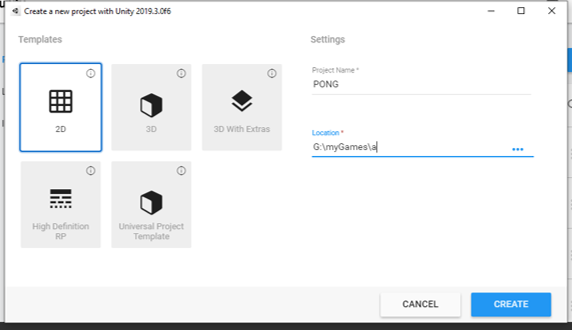
\includegraphics{Images/newproject.png}
\caption{New Project Settings}
\end{figure}

Now looking at the game Pong we should list first what we need to do.

\begin{itemize}
\tightlist
\item
  Draw shapes to the screen (paddles and ball)
\item
  Control 2D position of paddles based on input
\item
  Collision detection between paddles and ball to deflect ball back toward opponent
\item
  Collision detection between ball and map boundaries to keep ball within vertical bounds and to detect score (outside horizontal bounds)
\item
  Sound effects when ball hits paddles/walls or when a point is scored for flavor
\item
  Scorekeeping to determine winner
\end{itemize}

\hypertarget{drawing-shapes-to-the-screen}{%
\section{Drawing Shapes to the Screen}\label{drawing-shapes-to-the-screen}}

When you first start Unity, you should first arrange your workspace so that you can work more efficiently. First select \textbf{``Tall''} from the tab in the top right corner as seen in the image below.

\begin{figure}
\centering
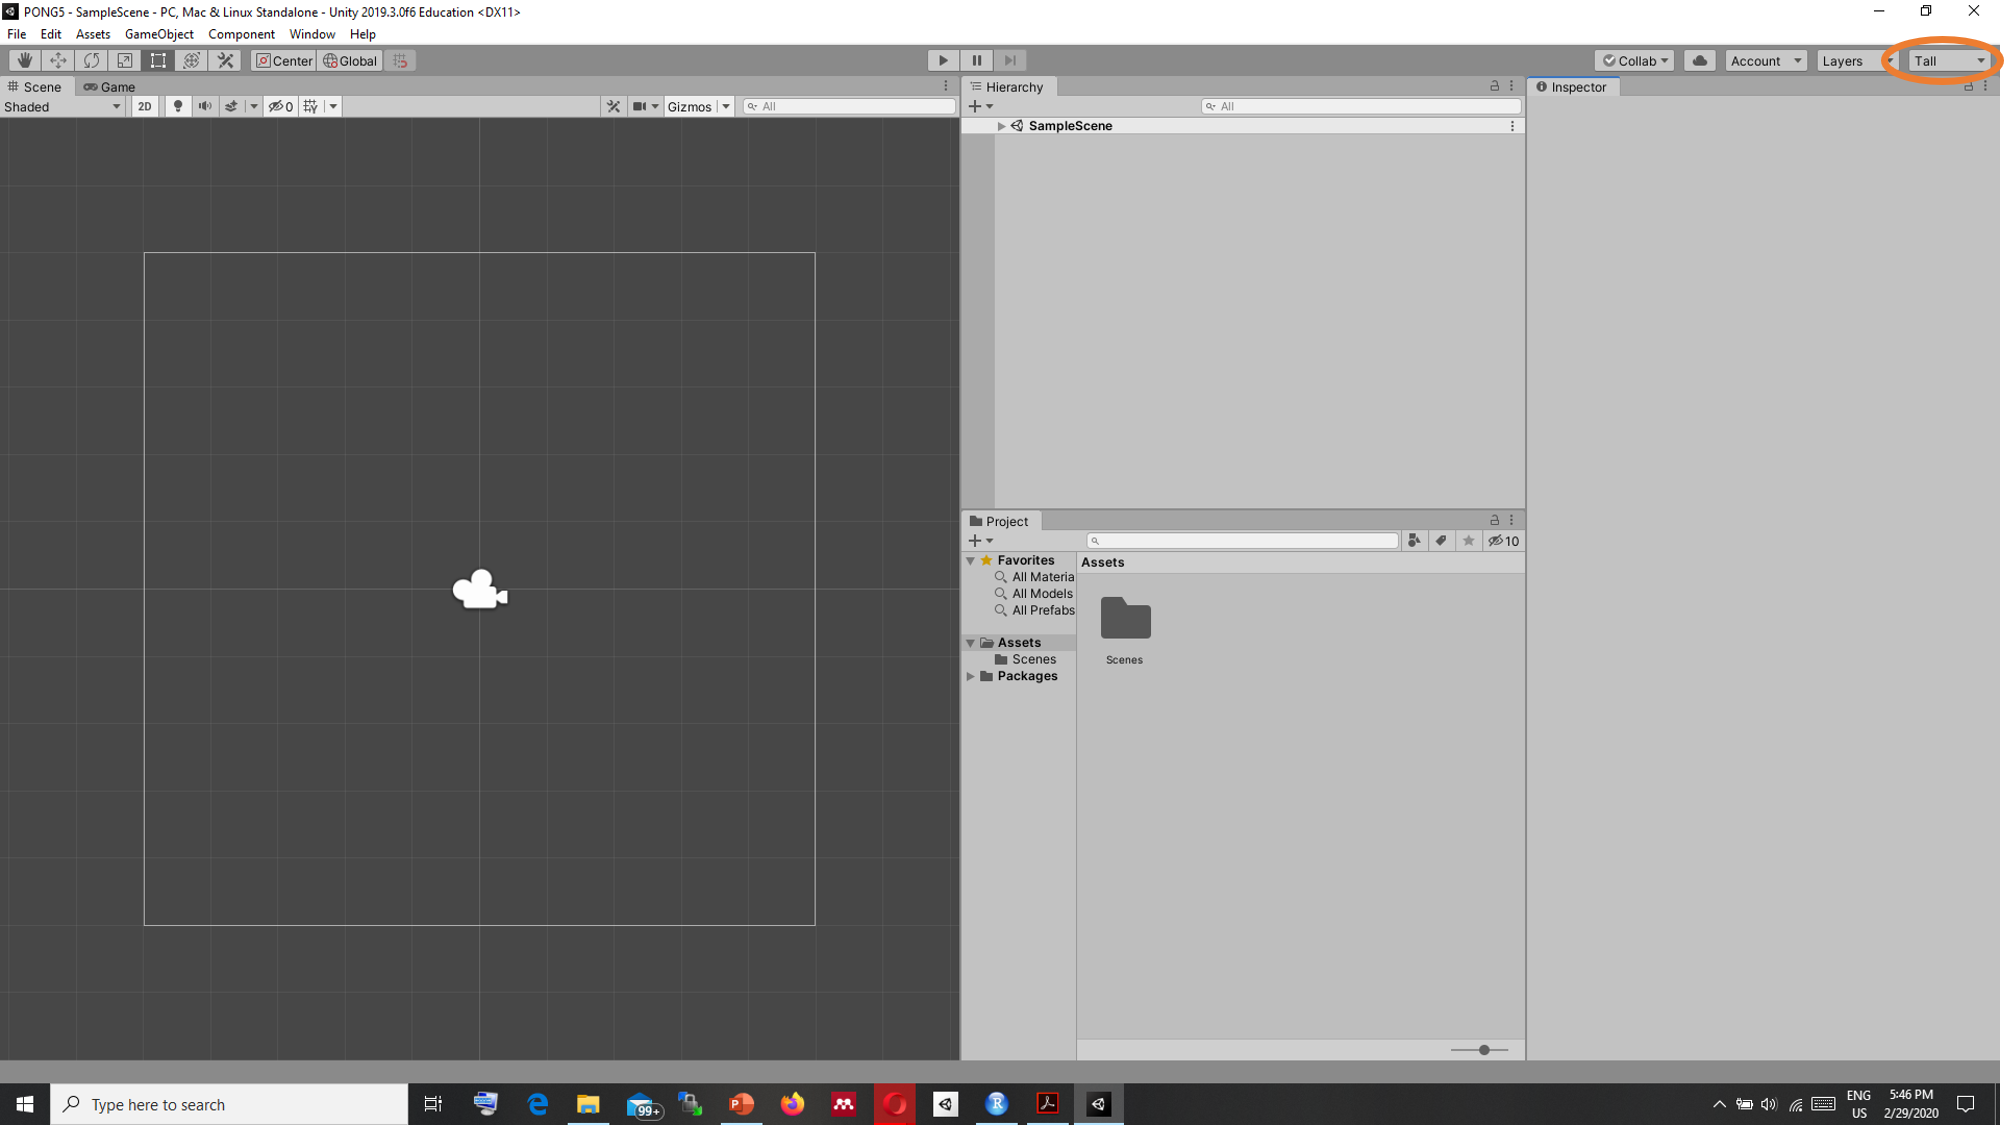
\includegraphics{Images/Setting.png}
\caption{Tall Workspace}
\end{figure}

You can drag the \textbf{Game window} to the bottom of the \textbf{Screen window} to have a workspace similar to the image.

\begin{figure}
\centering
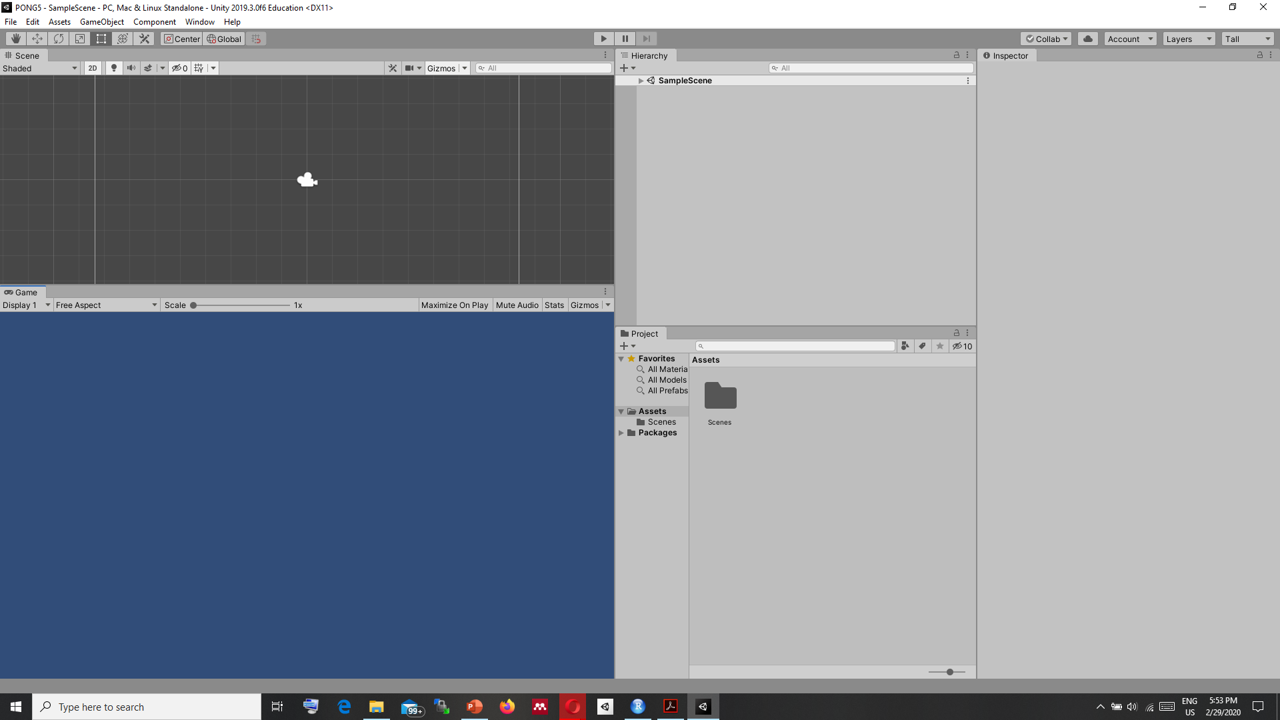
\includegraphics{Images/Setting2.png}
\caption{Professional Workspace}
\end{figure}

Now from the bottom of the \textbf{Game window} set the aspect ratio of the game. Aspect ratio adjusts the resolution of the game and ensures it looks same in all the devices.

Set the aspect ratio as Standalone 1024 X 768.

\begin{figure}
\centering
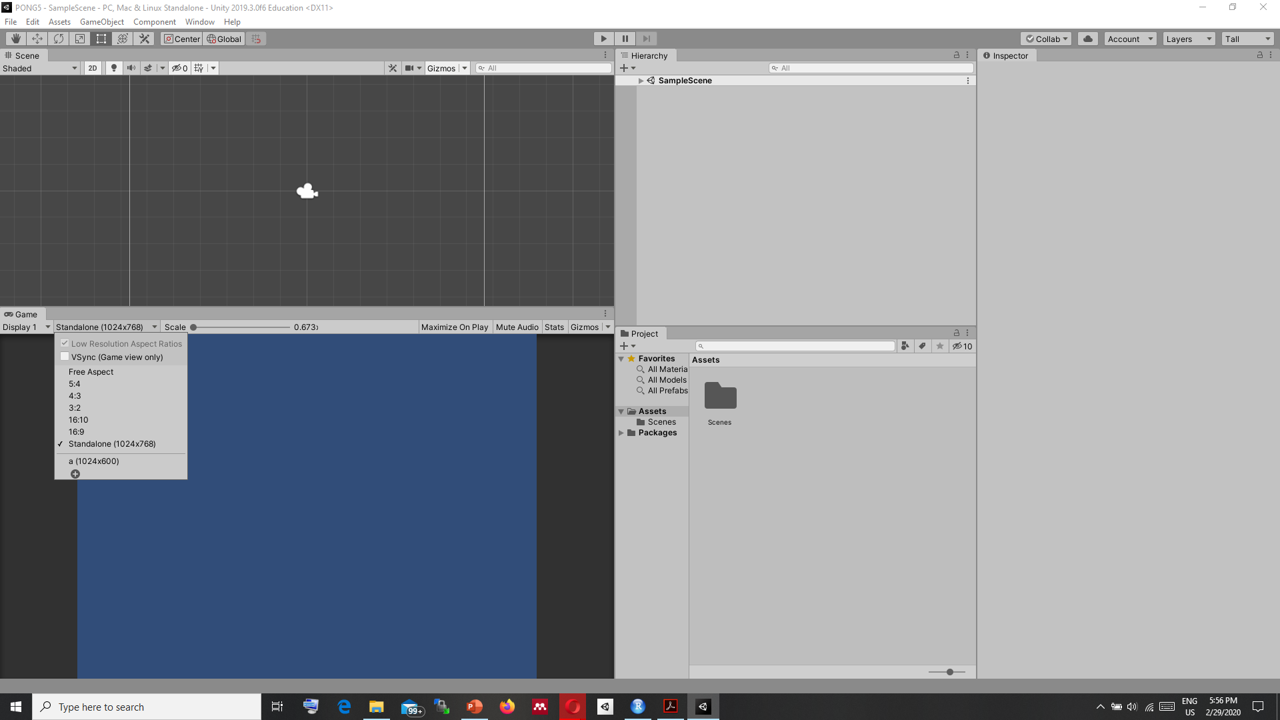
\includegraphics{Images/aspectRatio.png}
\caption{Aspect ratio -- Standalone 1024 x 768}
\end{figure}

Now in Unity window we have five windows open.

\begin{itemize}
\tightlist
\item
  Scene Window: Here we control the geometries that we are creating. You can manipulate objects here.
\item
  Game window: Here you play your games and inspect if everything works as expected.
\item
  Hierarchy: Here is the objects that are in the scenes.
\item
  Project: Project window holds your files such as assets, scripts etc.
\item
  Inspector: In the inspector window you can access properties of all object that you are manipulating.
\end{itemize}

First let's rename and save our scene. In the \textbf{Project window} select SampleScene and rename it as Game. After the change Unity will ask you to reload the scene.

Now we can click to camera and change the background color to black from the \textbf{Inspector window}.

\begin{figure}
\centering
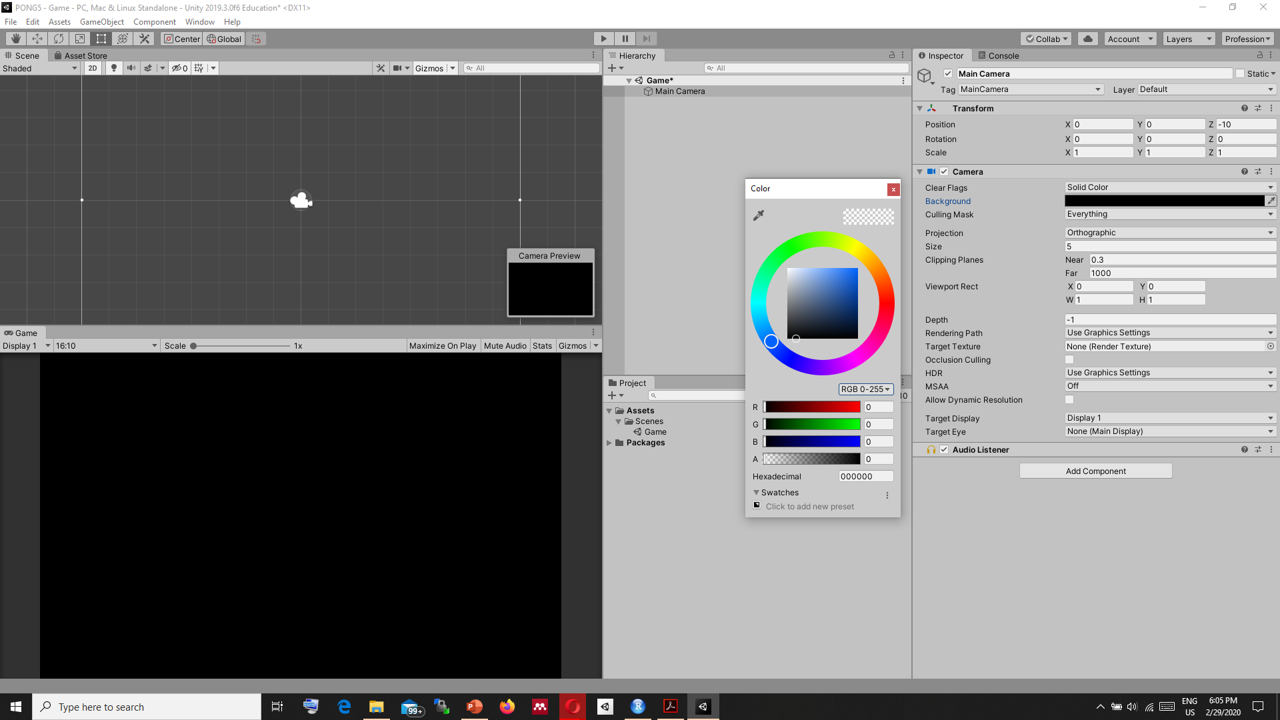
\includegraphics{Images/Backgrounf.png}
\caption{Changing the background color}
\end{figure}

Now, we are going to create the sprites that we will use in our game. Sprites are 2D graphics that are used in the games. For the two paddle and the ball used in the game we will use a square sprite.

Right click \textbf{Project window} from the menu click \textgreater Create\textgreater Sprites\textgreater Square

\begin{figure}
\centering
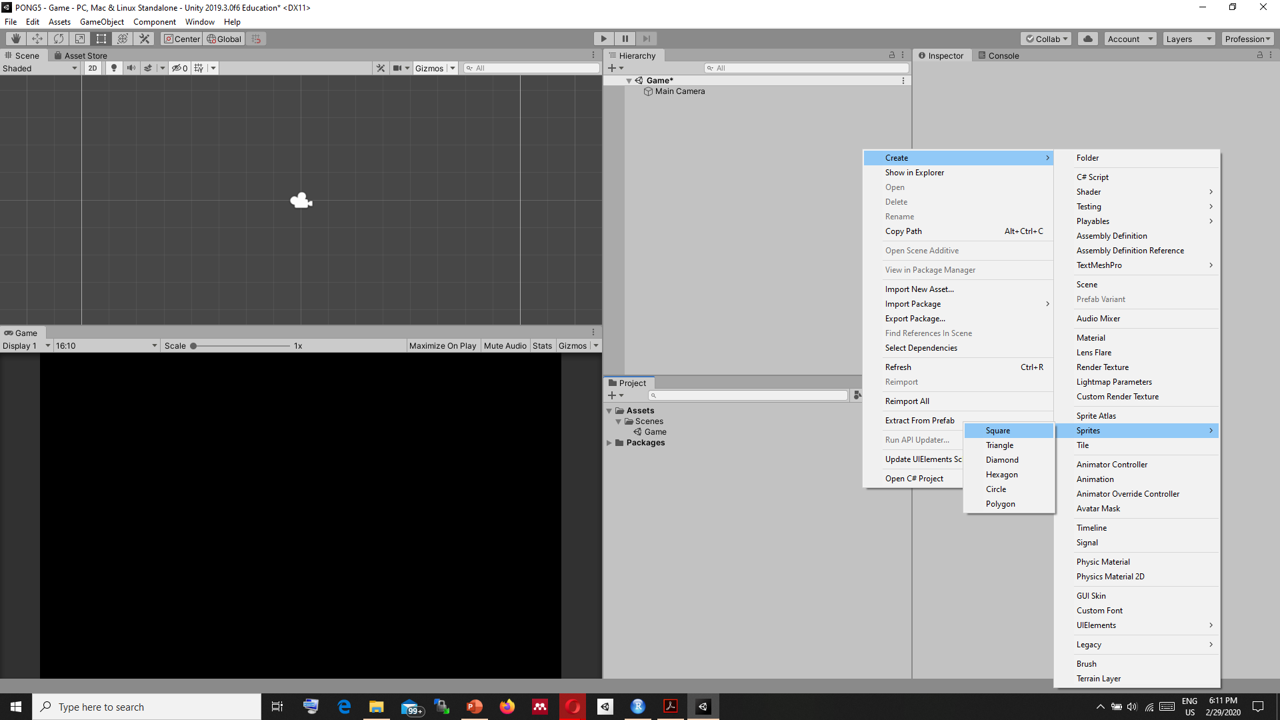
\includegraphics{Images/creatingSprite.png}
\caption{Creating a square sprite}
\end{figure}

We will create our players by using the square sprite. First drag square sprite into the hierarchy window and name it as Player 1.

\begin{figure}
\centering
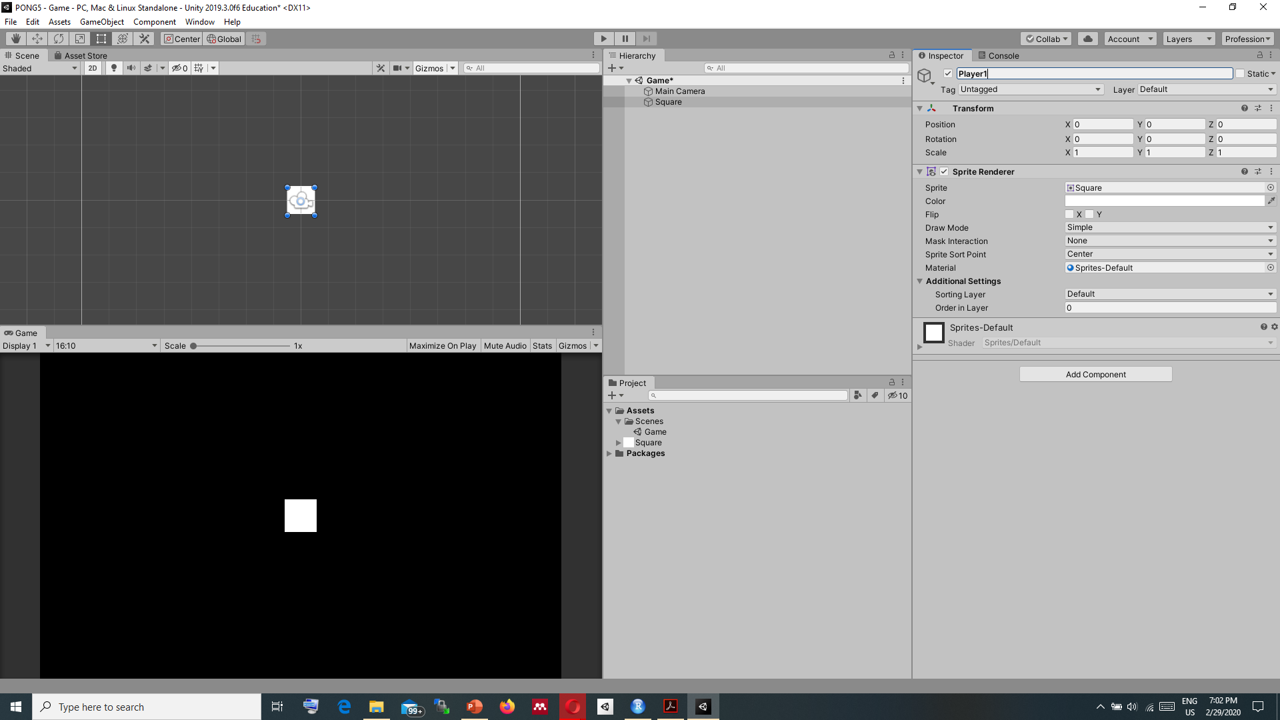
\includegraphics{Images/Player1.png}
\caption{Player1 sprite}
\end{figure}

Next, we need to scale the sprite so that it becomes a rectange. Select player 1 sprite and from the inspector window, set X scale to 0.5 and y scale to 2.

\begin{figure}
\centering
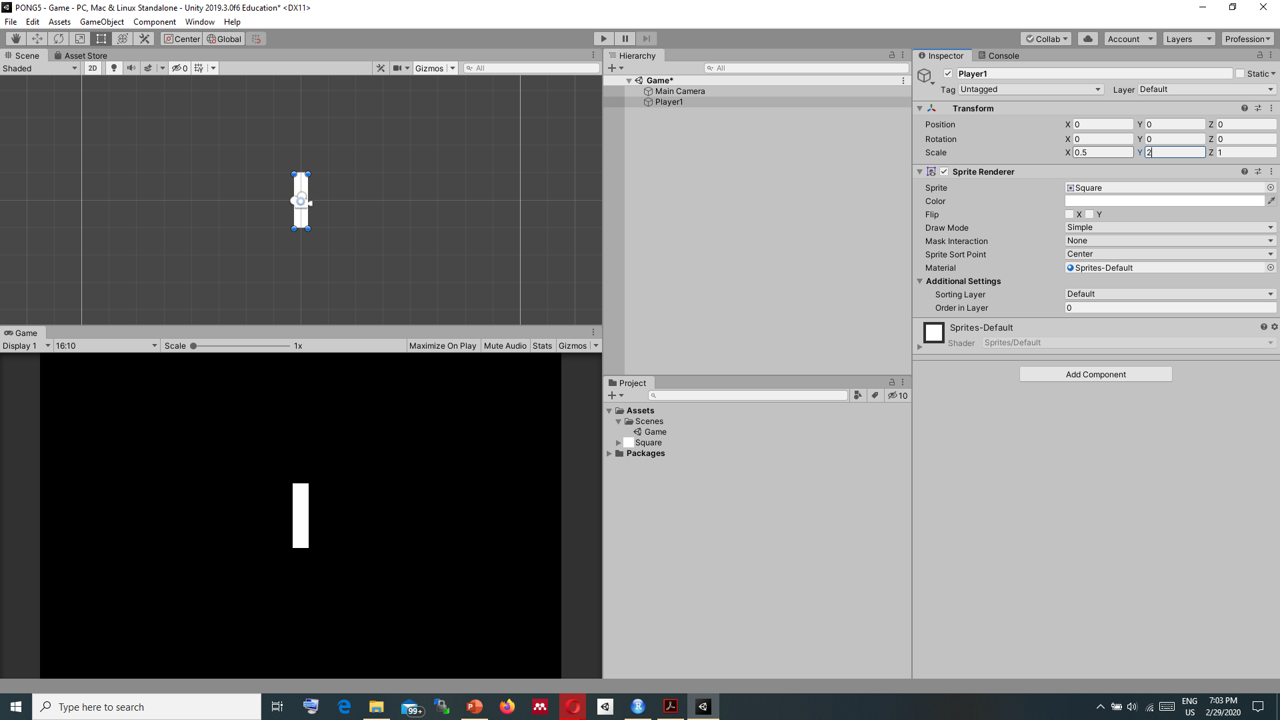
\includegraphics{Images/Player1-scale.png}
\caption{Scaling Player1 sprite}
\end{figure}

Player1 should be at the left side of the screen so let's change the position of the Player1. Set the X position to -6.4.

\begin{figure}
\centering
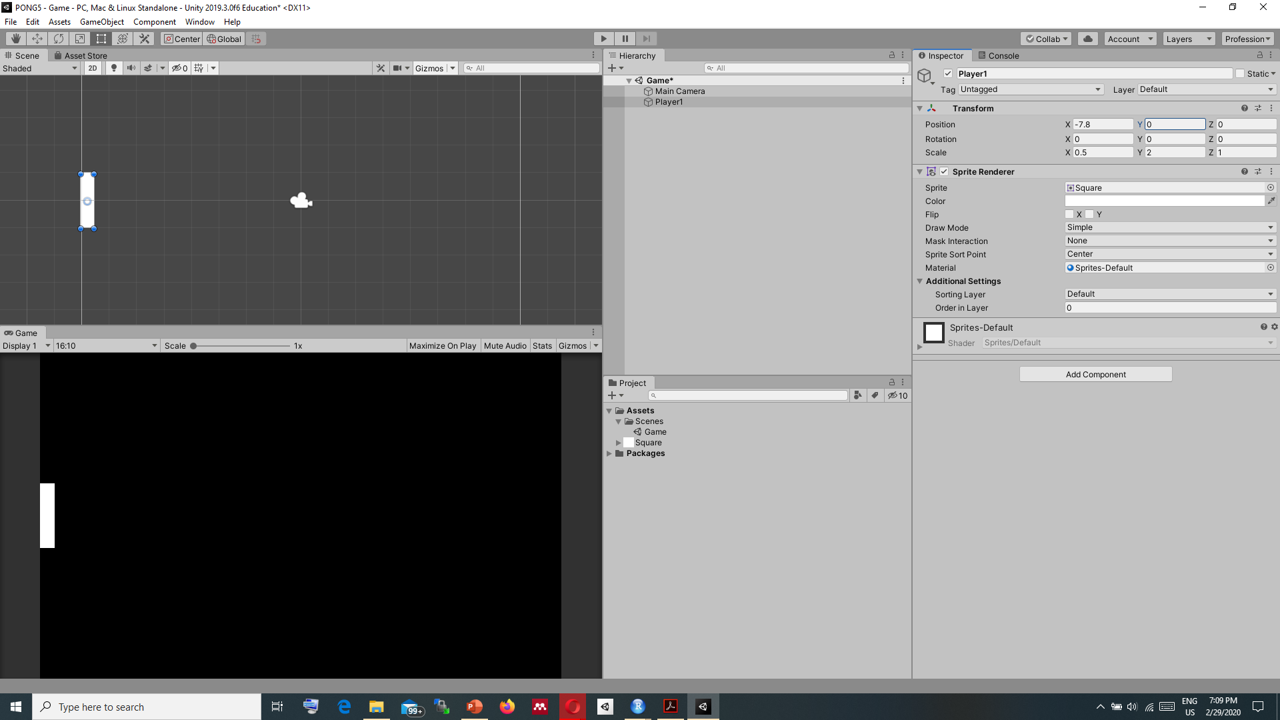
\includegraphics{Images/Player1-position.png}
\caption{Changing the location of Player1 sprite}
\end{figure}

Next, we should create Player 2. To do this, right click on Player 1 and select duplicate. From the inspector window, change the name to ``Player2'' and X position to 6.4 to move Player 2 to the right side of the screen.

\begin{figure}
\centering
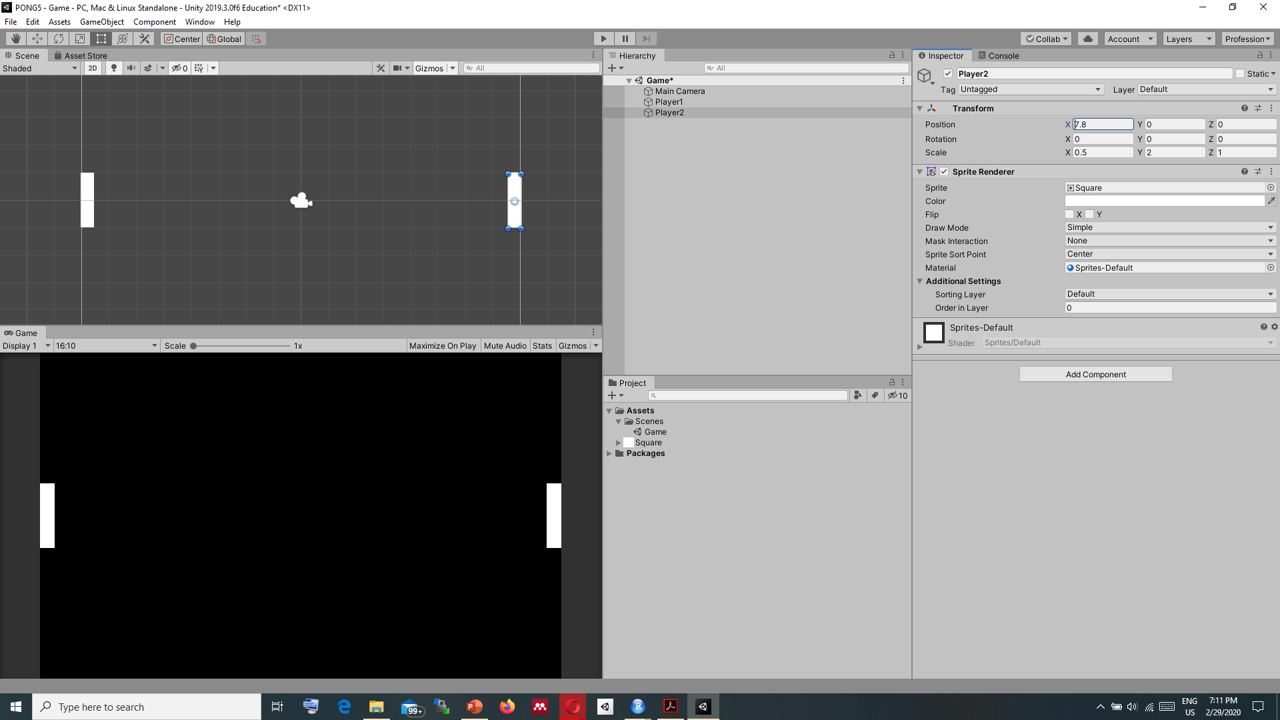
\includegraphics{Images/Player2.png}
\caption{Player2 sprite}
\end{figure}

Lastly, we should create the ball from the sprite. Drag square to \textbf{Hierarchy window}. Click over the sprite and change the name to ball. Next, change the scale of X and Y to 0.3.

\begin{figure}
\centering
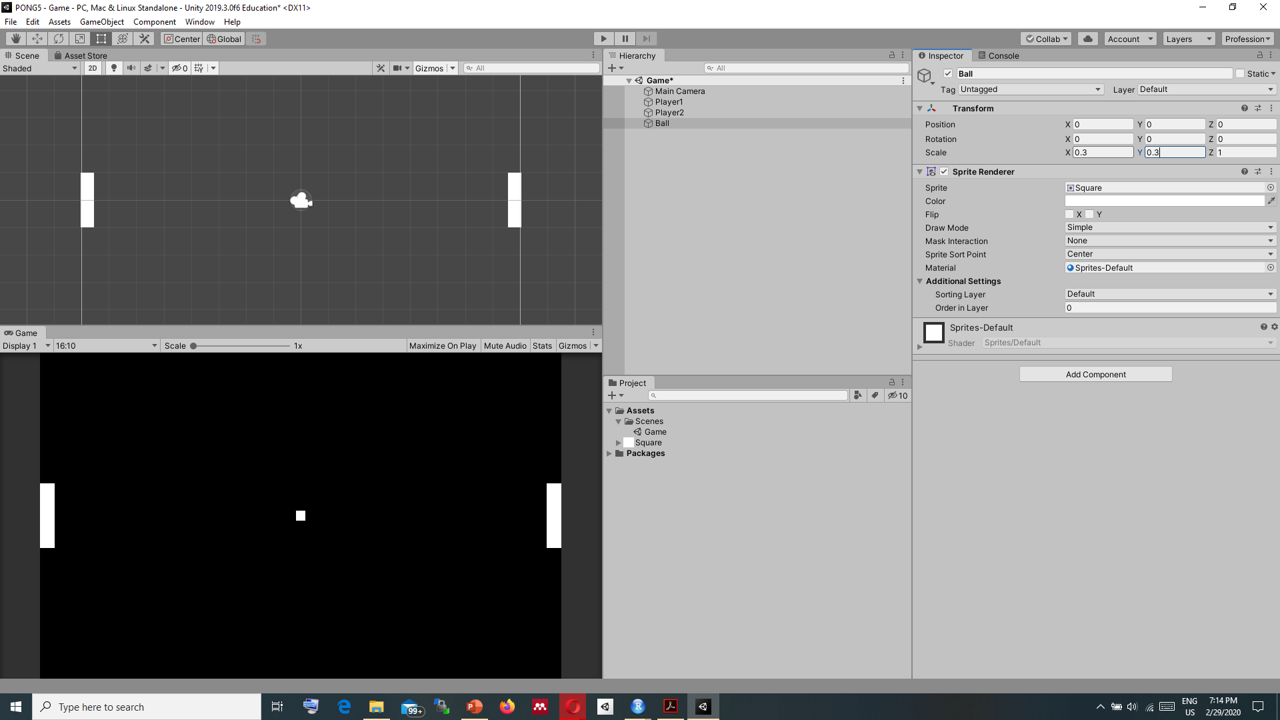
\includegraphics{Images/Ball.png}
\caption{Ball sprite}
\end{figure}

And to gather Player1 and Player2 in one folder create an empty GameObject by right clicking \textbf{Hierarchy window} \textgreater Create Empty.
Name it as Paddles and drag Player1 and Player2 into it.

\begin{figure}
\centering
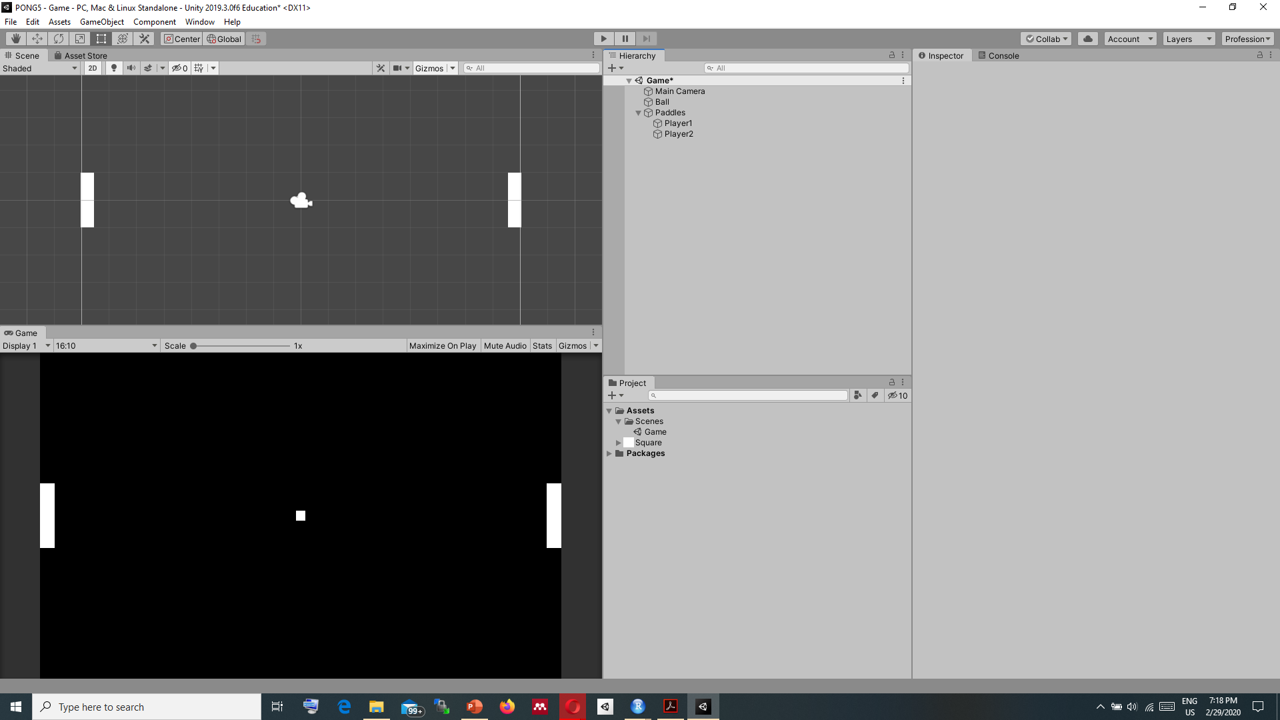
\includegraphics{Images/Paddles.png}
\caption{Empty Paddles GameObject}
\end{figure}

\hypertarget{user-input}{%
\section{User Input}\label{user-input}}

In the last step, we have created our paddles and the ball. However, they are static and they don't move with input. So let's connect the paddles to user input.

First, we should setup the controls to be used in the game.

From Edit Menu click \textgreater Edit\textgreater Project Settings.

Select Input Manager from the left side of the window. And duplicate Vertical Axes by right clicking over it.

\begin{figure}
\centering
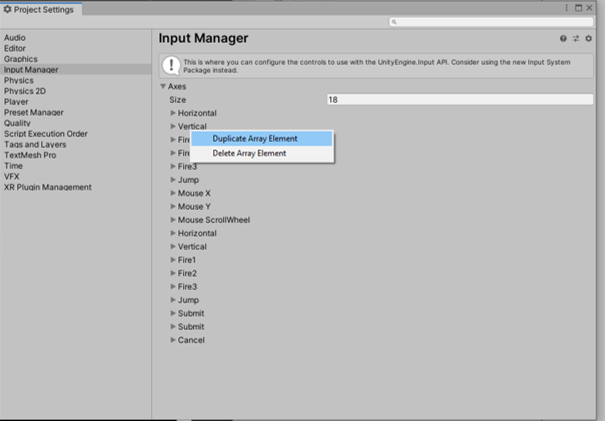
\includegraphics{Images/InputManager.png}
\caption{Duplicate Vertical Axes}
\end{figure}

Change the vertical Axes to Player1 by changing the name. Player1 will use w for up and s for down. So set the \textbf{Negative Button} as s and set \textbf{Positive Button} as w. Delete alt negative and alt positive buttons.

\begin{figure}
\centering
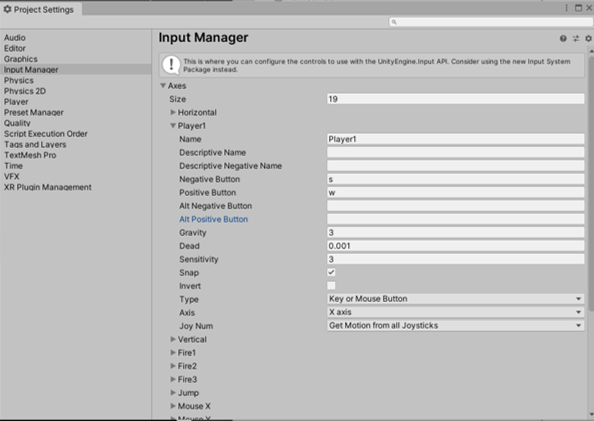
\includegraphics{Images/Player1controls.png}
\caption{Player1 controls w for up and s for down}
\end{figure}

Similarly, change the other vertical axes as Player2 and set the \textbf{Negative Button} as down and set \textbf{Positive Button} as up. Delete alt negative and alt positive buttons.

\begin{figure}
\centering
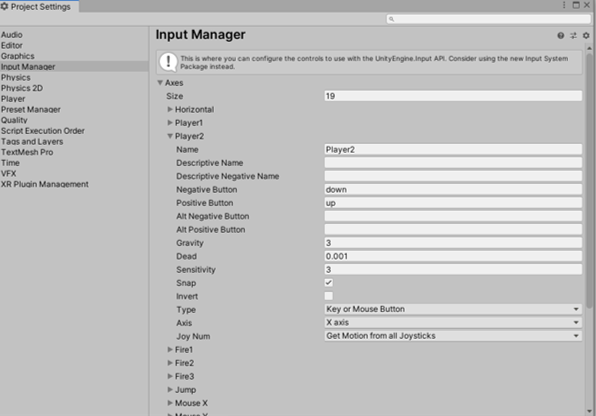
\includegraphics{Images/Player2controls.png}
\caption{Player1 controls up for up and down for down}
\end{figure}

To control the paddles using the input buttons we should create a C\# script. Right Click on Project Window and \textgreater Create\textgreater C\# Script

\begin{figure}
\centering
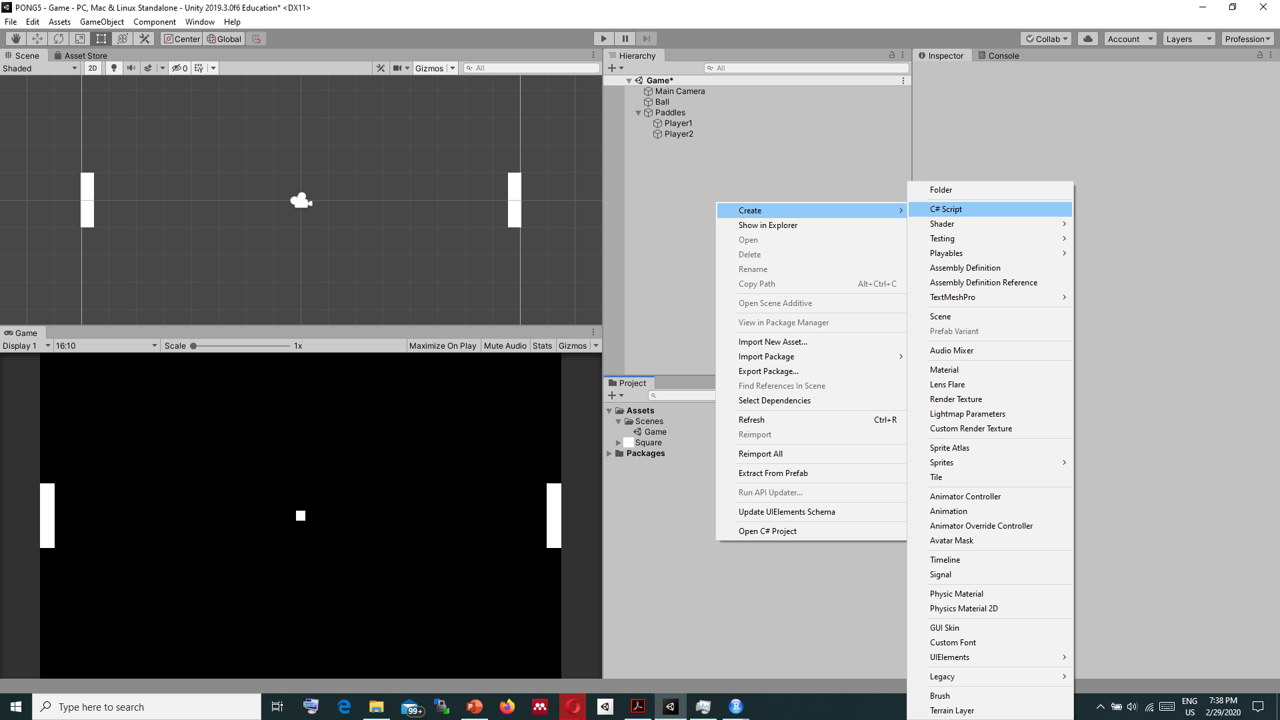
\includegraphics{Images/createScript.png}
\caption{Create Paddle Script}
\end{figure}

Name the script as Paddle and double click it. Double clicking a script file will bring up C\# editor. It can be Jetbrains rider or Visual Studio Code according to your installation.

First, we should setup our variables. We will use three variables.

\begin{itemize}
\tightlist
\item
  \_speed: holds the speed of the movement of the paddles
\item
  player1: refers GameObject of Player1
\item
  player2: refers GameObject of Player1
\end{itemize}

\begin{Shaded}
\begin{Highlighting}[]
\NormalTok{[SerializeField] }\KeywordTok{private} \DataTypeTok{float}\NormalTok{ _speed = 4f;}
\NormalTok{[SerializeField] GameObject player1;}
\NormalTok{[SerializeField] GameObject player2;}
\end{Highlighting}
\end{Shaded}

SerializeField in Unity means any variable that we have created will be accessible in the Unity interface. For more info: \url{https://docs.unity3d.com/ScriptReference/SerializeField.html}

After setting up our variable we can create Update() method.

\begin{Shaded}
\begin{Highlighting}[]
\CommentTok{// player1 - left player - movements}
\DataTypeTok{float}\NormalTok{ verticalInput1 = Input.}\FunctionTok{GetAxis}\NormalTok{(}\StringTok{"Player1"}\NormalTok{);}
\NormalTok{Vector3 direction1 = }\KeywordTok{new} \FunctionTok{Vector3}\NormalTok{(}\DecValTok{0}\NormalTok{, verticalInput1, }\DecValTok{0}\NormalTok{);}
\NormalTok{player1.}\FunctionTok{transform}\NormalTok{.}\FunctionTok{Translate}\NormalTok{(Time.}\FunctionTok{deltaTime}\NormalTok{ * _speed * direction1);}
\end{Highlighting}
\end{Shaded}

Here verticalInput1 receives the movement from the Player1 axes that we have created. According to the values we get, we create a direction1 vector3 which only receives values for Y axis since our player1 only moves up and down. And finally we move player1 every second.

We repeat the same code for player2:

\begin{Shaded}
\begin{Highlighting}[]
\CommentTok{// Player 2 - right player - movements }
\DataTypeTok{float}\NormalTok{ verticalInput2 = Input.}\FunctionTok{GetAxis}\NormalTok{(}\StringTok{"Player2"}\NormalTok{);}
\NormalTok{Vector3 direction2 = }\KeywordTok{new} \FunctionTok{Vector3}\NormalTok{(}\DecValTok{0}\NormalTok{, verticalInput2, }\DecValTok{0}\NormalTok{);}
\NormalTok{player2.}\FunctionTok{transform}\NormalTok{.}\FunctionTok{Translate}\NormalTok{(Time.}\FunctionTok{deltaTime}\NormalTok{ * _speed * direction2);}
\end{Highlighting}
\end{Shaded}

Now we need to associate Paddle script with PaddleS folder we have created. Drag the Paddle script from the \textbf{Project Window} to \textbf{Hierarchy Window} and drop it over the Paddles folder. Click on the Paddles folder and from the inspector window check if you can see Paddle (Script). Now drag Player1 from the \textbf{Hierarchy Window} to Player1 in Inspector and repeat this for Player2.

\begin{figure}
\centering
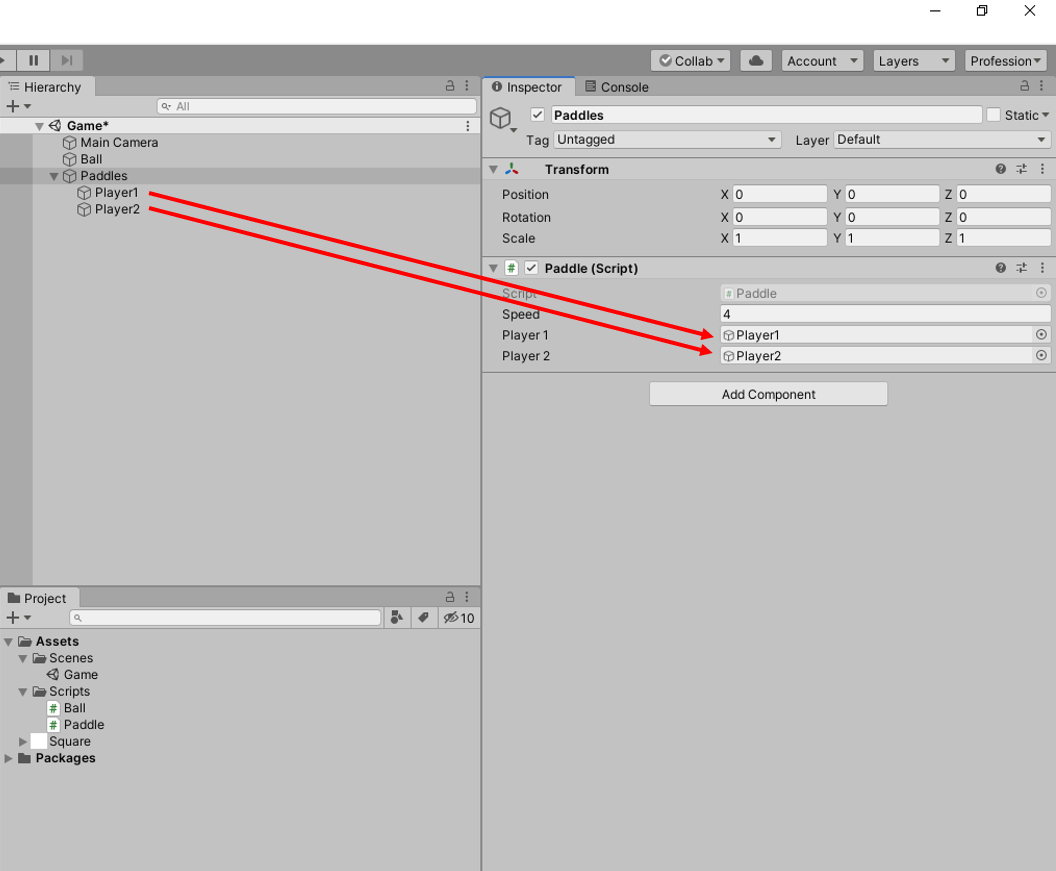
\includegraphics{Images/AssociateScript.png}
\caption{Associate the script with Paddles}
\end{figure}

Finally, if we click the play button, the game starts and we can control our paddles.

\begin{figure}
\centering
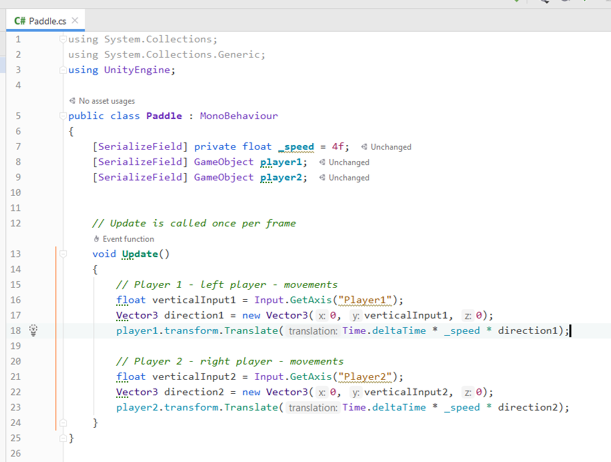
\includegraphics{Images/PaddleScript.png}
\caption{Paddle Script with the controls}
\end{figure}

\hypertarget{player-bounds}{%
\section{Player Bounds}\label{player-bounds}}

In the last section, we set up movements with the keyboard input. However, the paddles can go out of the bounds of the game space. We need to restrict the movement of the paddles to the screen size.

To achieve this we need to include two \textbf{if} statements to check if the paddles are at the top or bottom of the screen.

\begin{Shaded}
\begin{Highlighting}[]
\KeywordTok{if}\NormalTok{ (player1.}\FunctionTok{transform}\NormalTok{.}\FunctionTok{position}\NormalTok{.}\FunctionTok{y}\NormalTok{ < }\FloatTok{-3.9}\NormalTok{ && verticalInput1 < }\DecValTok{0}\NormalTok{)}
\NormalTok{\{}
\NormalTok{  verticalInput1 = }\DecValTok{0}\NormalTok{;}
\NormalTok{\}}
\KeywordTok{else} \KeywordTok{if}\NormalTok{ (player1.}\FunctionTok{transform}\NormalTok{.}\FunctionTok{position}\NormalTok{.}\FunctionTok{y}\NormalTok{ > }\FloatTok{3.9}\NormalTok{ && verticalInput1 > }\DecValTok{0}\NormalTok{)}
\NormalTok{\{}
\NormalTok{  verticalInput1 = }\DecValTok{0}\NormalTok{;}
\NormalTok{\}}
\end{Highlighting}
\end{Shaded}

Here the first if clause checks if player1's position is at the top of the screen which is -3.9, if it then the code sets the speed of the paddle to 0 which stops the movement. Similarly there is an another if statement which checks if player1 is at the bottom of the screen and again this also stops the paddle which ensures the paddle stays inside the screen.

We need to do the same check for player2 which makes the code like below.

\begin{figure}
\centering
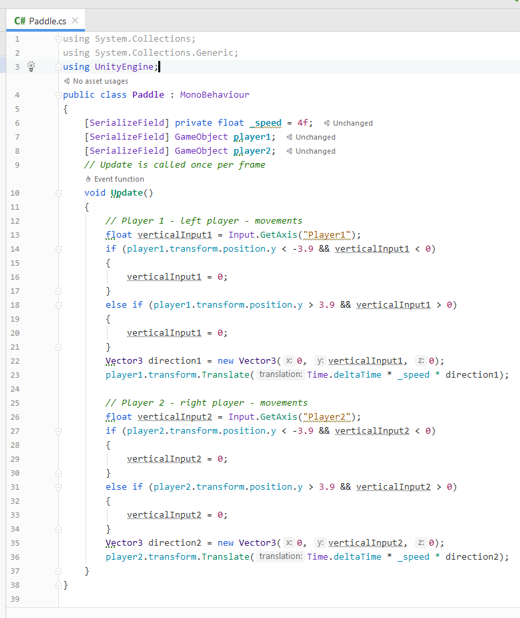
\includegraphics{Images/Bounds.png}
\caption{Script change to keep paddles inside the screen}
\end{figure}

\hypertarget{ball-movement}{%
\section{Ball Movement}\label{ball-movement}}

Now, we should make the ball move. For this we will create a ball script. Right click the \textbf{Project Window} \textgreater Create\textgreater C\# Script and name it as ball.

To make it tidier in the Project Window, create a folder and name it as Scripts and put Ball and Paddle script inside the Scripts folder.

We should start the game by hitting a key which will serve the ball. First, we should set the variables:

\begin{Shaded}
\begin{Highlighting}[]
\NormalTok{[SerializeField] }\KeywordTok{private} \DataTypeTok{float}\NormalTok{ _speed = 4f;}
\KeywordTok{private} \DataTypeTok{bool}\NormalTok{ serve = }\KeywordTok{true}\NormalTok{;  }\CommentTok{// boolean to indicate serve action}
\KeywordTok{private} \DataTypeTok{bool}\NormalTok{ end = }\KeywordTok{false}\NormalTok{;  }\CommentTok{// game ends}
\KeywordTok{private}\NormalTok{ Vector3 direction; }\CommentTok{// direction of the ball}
\end{Highlighting}
\end{Shaded}

\begin{itemize}
\tightlist
\item
  \_speed: controls the speed of the ball.
\item
  serve: Indicates the serve state
\item
  end: indicates the end state which ends the game
\item
  direction: direction of the ball as Vector3
\end{itemize}

Next we should create our code, if the state is serve and someone presses Enter the ball should start moving in a random direction.

\begin{Shaded}
\begin{Highlighting}[]
\KeywordTok{if}\NormalTok{ (Input.}\FunctionTok{GetKeyDown}\NormalTok{(KeyCode.}\FunctionTok{Return}\NormalTok{) && serve)}
\NormalTok{\{}
\NormalTok{  direction = }\KeywordTok{new} \FunctionTok{Vector3}\NormalTok{(Random.}\FunctionTok{Range}\NormalTok{(-}\FloatTok{4.0f}\NormalTok{, 4f), Random.}\FunctionTok{Range}\NormalTok{(-}\FloatTok{8.0f}\NormalTok{, 8f), }\DecValTok{0}\NormalTok{);}
\NormalTok{  serve = }\KeywordTok{false}\NormalTok{;}
\NormalTok{\}}
\KeywordTok{if}\NormalTok{ (!serve)}
\NormalTok{\{}
\NormalTok{  transform.}\FunctionTok{Translate}\NormalTok{(Time.}\FunctionTok{deltaTime}\NormalTok{ * _speed * direction);}
\NormalTok{\}}
\end{Highlighting}
\end{Shaded}

After creating this script, we should drag the ball script over the ball GameObject. If we start the game, with a press to Return key the ball starts moving. However, since we did not set up the boundary to the ball it goes out of bounds.

\begin{figure}
\centering
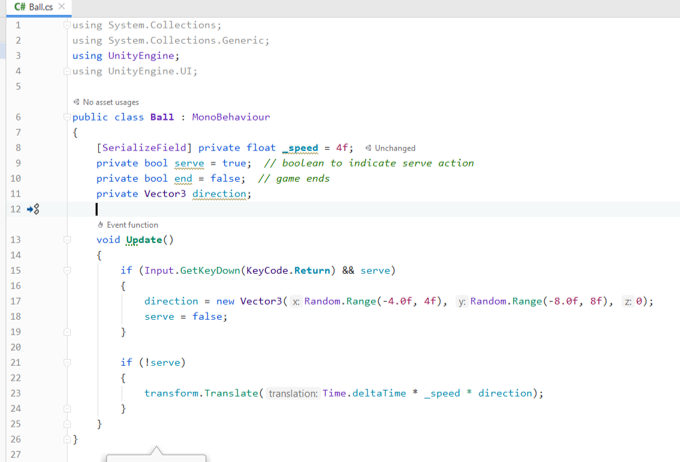
\includegraphics{Images/BallScript.png}
\caption{Ball Script}
\end{figure}

Next we will set up the boundary for the ball to bounce from the sides of the screen.

\hypertarget{bouncing-from-the-sides}{%
\section{Bouncing from the sides}\label{bouncing-from-the-sides}}

For this the y position of the ball should be between -4.8 and 4.8. We will put two if conditionals; if the y position of the ball is bigger than 4.8, ball's direction should flip in the y direction. Similarly, if the y position of the ball is lesser than -4.8 ball's direction should flip in the y direction as well.

\begin{Shaded}
\begin{Highlighting}[]
\KeywordTok{if}\NormalTok{ (transform.}\FunctionTok{position}\NormalTok{.}\FunctionTok{y}\NormalTok{ > }\FloatTok{4.8}\NormalTok{ && direction.}\FunctionTok{y}\NormalTok{ > }\DecValTok{0}\NormalTok{)}
\NormalTok{\{}
\NormalTok{  direction.}\FunctionTok{y}\NormalTok{ = -direction.}\FunctionTok{y}\NormalTok{;}
\NormalTok{\}}
\KeywordTok{if}\NormalTok{ (transform.}\FunctionTok{position}\NormalTok{.}\FunctionTok{y}\NormalTok{ < }\FloatTok{-4.8}\NormalTok{ && direction.}\FunctionTok{y}\NormalTok{ < }\DecValTok{0}\NormalTok{)}
\NormalTok{\{}
\NormalTok{  direction.}\FunctionTok{y}\NormalTok{ = -direction.}\FunctionTok{y}\NormalTok{;}
\NormalTok{\}}
\end{Highlighting}
\end{Shaded}

By adding these clauses will ensure that the ball stays in the boundary of the screen.

\begin{figure}
\centering
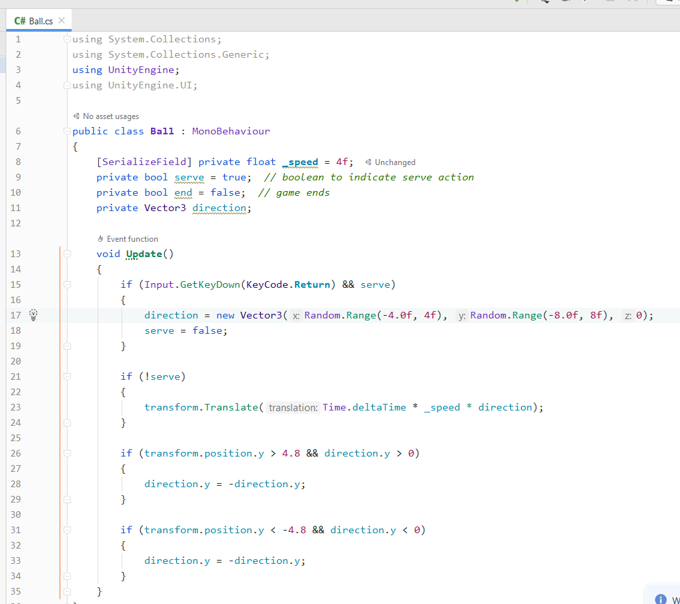
\includegraphics{Images/BallBoundary.png}
\caption{Keep the ball inside the boundary}
\end{figure}

\hypertarget{collider-for-ball-and-paddles}{%
\section{Collider for Ball and Paddles}\label{collider-for-ball-and-paddles}}

The game is still not playable since it does not collide with the paddles. We should add rigidbody2d and box collider to the player1 \& player2 gameObjects and to the ball gameobject. To add rigidbody2d to player1, we click on the player1 in the \textbf{Hierarchy Window} and from the \textbf{Inspector Window} we click on add component and type rigidbody2d.

\begin{figure}
\centering
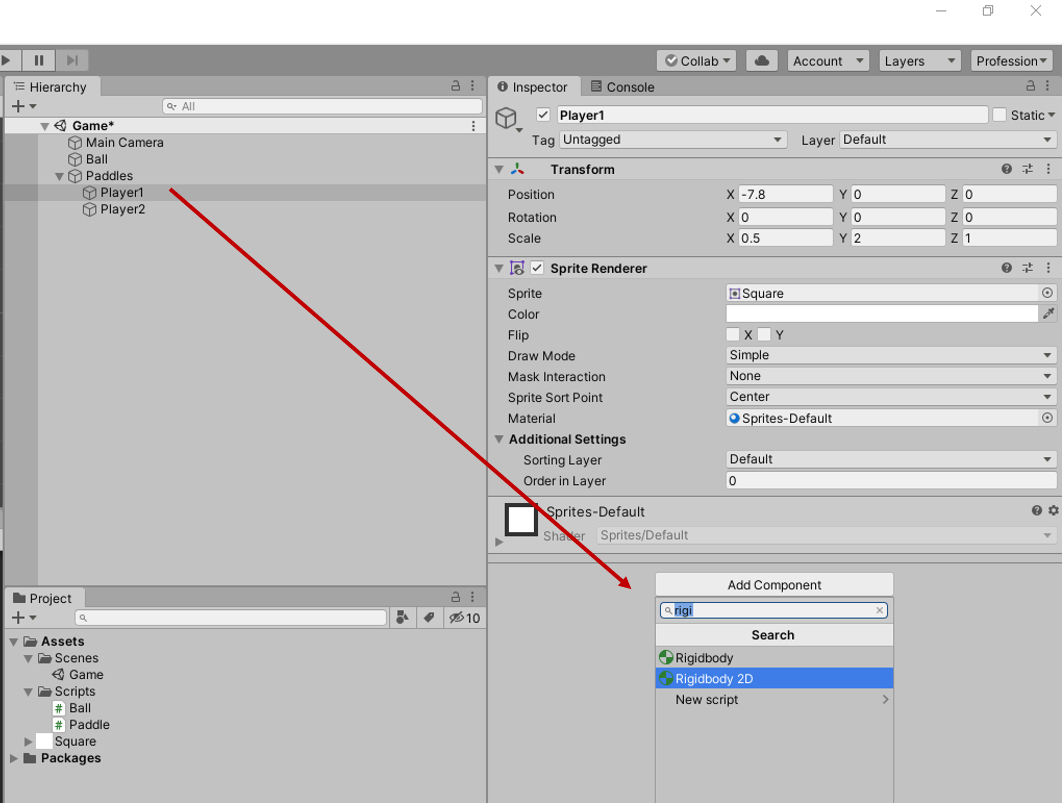
\includegraphics{Images/AddComponent.png}
\caption{Add Component}
\end{figure}

In the rigidbody2d, in Body Type tab select Kinematic. Kinematic ensures there is no gravity and all the movements occur according to our control.

\begin{figure}
\centering
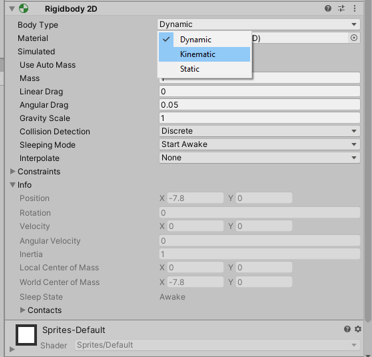
\includegraphics{Images/Rigidbody2d.png}
\caption{Rigidbody2 - Kinematic}
\end{figure}

After adding rigidbody2d to all three gameObjects, we should add boxCollider2d for them as well. From the same place that we added rigidbody2d this time we add boxcollider2d.

\begin{figure}
\centering
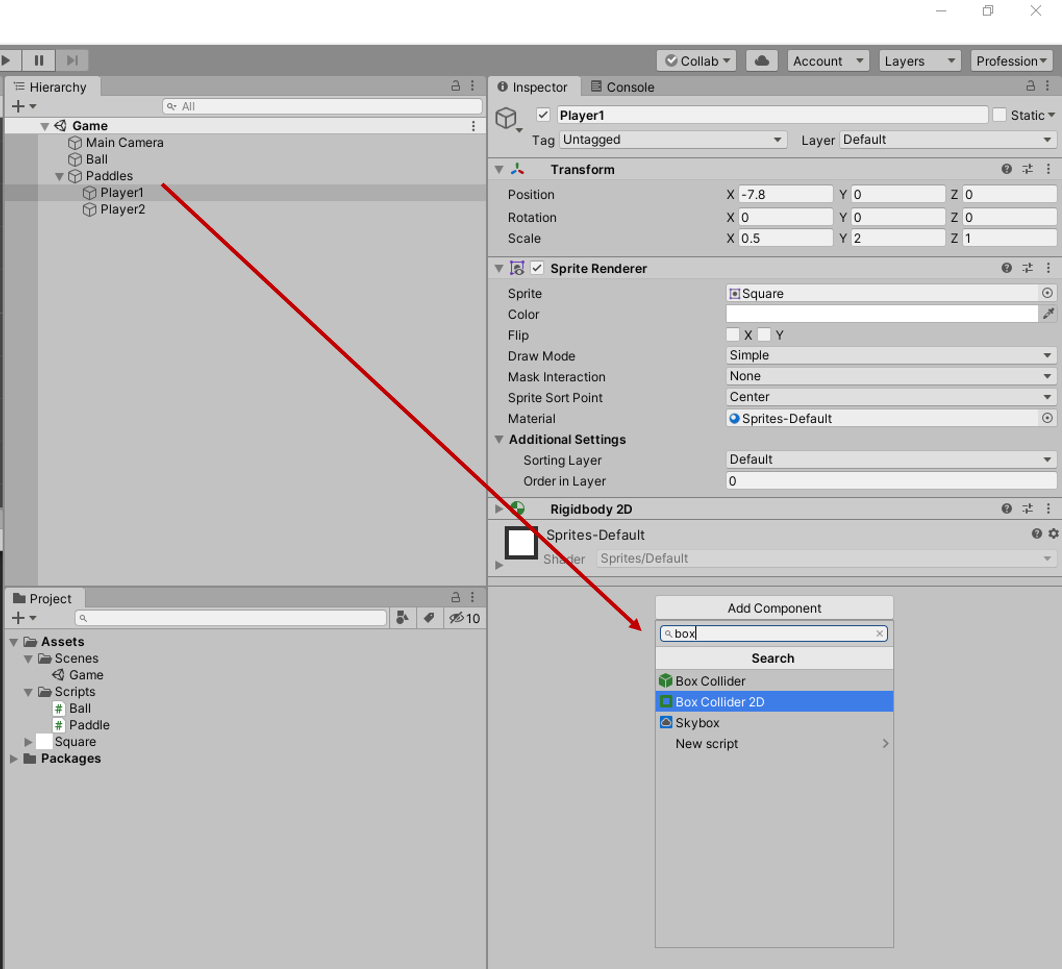
\includegraphics{Images/BoxCollider2d.png}
\caption{BoxCollider2D}
\end{figure}

In the BoxCollider2d menu we should select IsTrigger option.

\begin{figure}
\centering
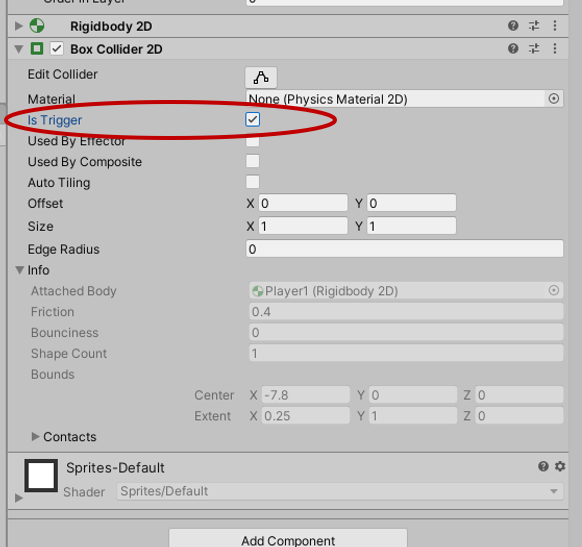
\includegraphics{Images/IsTrigger.png}
\caption{Is Trigger}
\end{figure}

After adding rigidbody2d and boxcollider2d, now we should handle the code. Openning up ball script, we create OnTriggerEnter2D method. This methods calls up when two objects collide.

\begin{Shaded}
\begin{Highlighting}[]
\KeywordTok{private} \DataTypeTok{void} \FunctionTok{OnTriggerEnter2D}\NormalTok{(Collider2D other)}
\NormalTok{\{}
\NormalTok{  direction.}\FunctionTok{x}\NormalTok{ = -direction.}\FunctionTok{x}\NormalTok{;}
\NormalTok{\}}
\end{Highlighting}
\end{Shaded}

This is a very simple method. It flips the direction of the ball when there is a collision between the ball and the paddle. So the new ball script is:

\begin{figure}
\centering
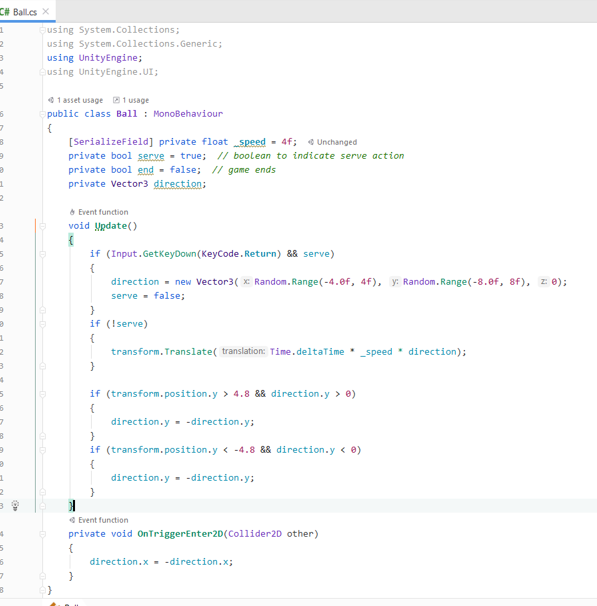
\includegraphics{Images/BallScript2.png}
\caption{Updated Ball Script}
\end{figure}

\hypertarget{score}{%
\section{Score}\label{score}}

Next, we should be able to determine if there is a score and reset the game if there is a score, starting the game from the center of the screen with a key press again.

To keep up the score we create two new variables:

\begin{Shaded}
\begin{Highlighting}[]
\KeywordTok{private} \DataTypeTok{int}\NormalTok{ player1Score = }\DecValTok{0}\NormalTok{;}
\KeywordTok{private} \DataTypeTok{int}\NormalTok{ player2Score = }\DecValTok{0}\NormalTok{;}
\end{Highlighting}
\end{Shaded}

We will include a code to check the position of the ball and if the ball's position is lesser than -6.7, means the ball has left the screen from the left thus player2 wins a score. If that happens we call the reset method and increase player2 score. If the score is 15 then the game ends, else the ball is returned to the center to be served again,

\begin{Shaded}
\begin{Highlighting}[]
\KeywordTok{if}\NormalTok{ (transform.}\FunctionTok{position}\NormalTok{.}\FunctionTok{x}\NormalTok{ < }\FloatTok{-6.7}\NormalTok{)}
\NormalTok{\{}
\NormalTok{  player2Score++;}
  \FunctionTok{Reset}\NormalTok{();}
  \KeywordTok{if}\NormalTok{ (player2Score == }\DecValTok{15}\NormalTok{)}
\NormalTok{  \{}
\NormalTok{    end = }\KeywordTok{true}\NormalTok{;}
\NormalTok{  \} }\KeywordTok{else}\NormalTok{ \{serve = }\KeywordTok{true}\NormalTok{;\}}
\NormalTok{\}}
\end{Highlighting}
\end{Shaded}

Reset method just centers the ball.

\begin{Shaded}
\begin{Highlighting}[]
\KeywordTok{private} \DataTypeTok{void} \FunctionTok{Reset}\NormalTok{()}
\NormalTok{\{}
\NormalTok{  transform.}\FunctionTok{position}\NormalTok{ = }\KeywordTok{new} \FunctionTok{Vector3}\NormalTok{(}\DecValTok{0}\NormalTok{,}\DecValTok{0}\NormalTok{,}\DecValTok{0}\NormalTok{);}
\NormalTok{\}}
\end{Highlighting}
\end{Shaded}

After adding these codes and repeating the process for the right side, we have the scoring component of the game.

\hypertarget{score-update-and-ui}{%
\section{Score update and UI}\label{score-update-and-ui}}

Next we need to show the scores in User Interface (UI). For this we need to Add Text to the Screen.

Right clicking \textbf{Hierarchy Window}, select \textgreater Create\textgreater UI\textgreater Text.

\begin{figure}
\centering
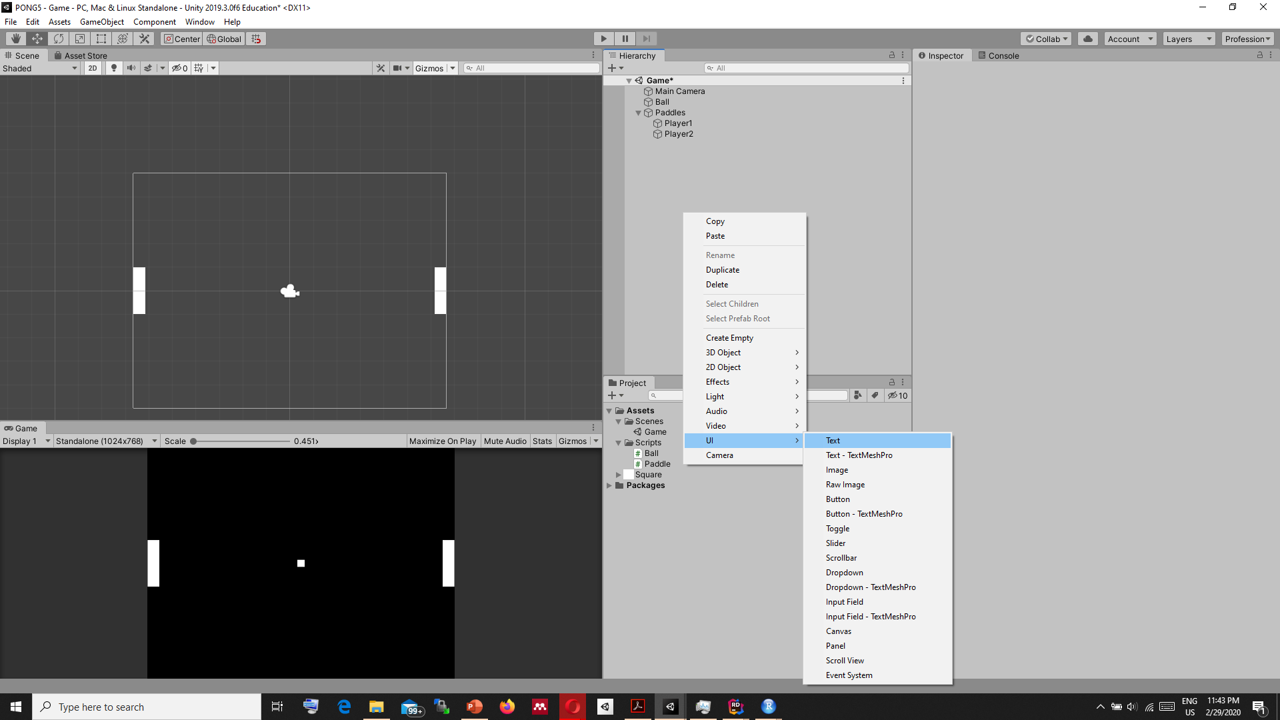
\includegraphics{Images/UIText.png}
\caption{Adding UI Text}
\end{figure}

We should first name the UI Text as Player1ScoreText.Next we click on the anchor icon and select top, center. And adjust PosX as -150, Pos Y as -100, Text as 0, Font Size as 100, Horizontal Overflow as overflow and Vertical Overflow as overflow as in the image below.

\begin{figure}
\centering
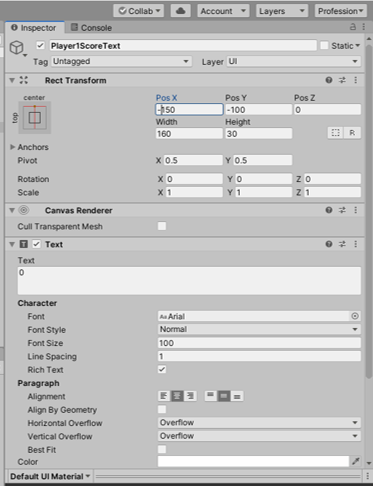
\includegraphics{Images/Player1ScoreText.png}
\caption{Setting Up Player 1 Score Text}
\end{figure}

We should do the same for Player2, so right click on it and duplicate. Change its name as Player2ScoreText and PosX as 150.

After this step, we should associate this text and use it in our ball script. So we should add following variables to the code:

\begin{Shaded}
\begin{Highlighting}[]
\NormalTok{[SerializeField] }\KeywordTok{private}\NormalTok{ Text player1ScoreText;}
\NormalTok{[SerializeField] }\KeywordTok{private}\NormalTok{ Text player2ScoreText;}
\end{Highlighting}
\end{Shaded}

And these fields should be updated each time there is a score so we add the following code after the Reset function call.

\begin{Shaded}
\begin{Highlighting}[]
\NormalTok{player2ScoreText.}\FunctionTok{text}\NormalTok{ =  player2Score.}\FunctionTok{ToString}\NormalTok{();}
\end{Highlighting}
\end{Shaded}

After adding these two code snippets we should click on Ball gameobject and drag Player1ScoreText and Player2ScoreText to its places.

Finally, our game mechanics works, next we will add sound that plays when there is a collision between the ball and the paddles.

\hypertarget{sound}{%
\section{Sound}\label{sound}}

For the sound, you should download the sound file from Github. Place the paddle\_hit file inside the assets folder. Drag the file into the \textbf{Hierarchy window}.

Add a variable in ball script.

\begin{Shaded}
\begin{Highlighting}[]
\NormalTok{[SerializeField] }\KeywordTok{private}\NormalTok{ AudioSource _paddleHit;}
\end{Highlighting}
\end{Shaded}

Add the code that plays the sound when there is a collision between the paddles and the ball inside the OnTriggerEnter2D method.

\begin{Shaded}
\begin{Highlighting}[]
\NormalTok{_paddleHit.}\FunctionTok{Play}\NormalTok{();}
\end{Highlighting}
\end{Shaded}

Select the ball gameObject from the \textbf{Hierarchy Window} and drag the paddle\_hit file to its place in ball script.

Now the game is ready, play it and enjoy your first game.

\hypertarget{assignment}{%
\section{Assignment}\label{assignment}}

Now I want you to improve 5 aspects of the game. Some ideas:

\begin{itemize}
\tightlist
\item
  Change background color, add texture etc.
\item
  Change colors/textures etc. of paddles
\item
  Change some mechanics, the ball gets faster each time etc.
\item
  Add AI to control the paddle -- bonus points, hard option
\end{itemize}

To submit your work, you need to commit your changes to Github and send me a link of your username and project.

\hypertarget{flappy-bird}{%
\chapter{Flappy Bird}\label{flappy-bird}}

Flappy Bird is a mobile game developed by Vietnamese video game artist and programmer Dong Nguyen, under his game development company dotGears. The game is a side-scroller where the player controls a bird, attempting to fly between columns of green pipes without hitting them.

\begin{figure}
\centering
\includegraphics{Images/flappy.gif}
\caption{Flappy Bird}
\end{figure}

In this course we are going to build Flappy Bird in UNITY.

\hypertarget{initial-setup}{%
\section{Initial Setup}\label{initial-setup}}

Setting up the aspect ratio

\hypertarget{critical-game-analysis}{%
\chapter{Critical Game Analysis}\label{critical-game-analysis}}

I am going to briefly cover how to do a critical game analysis. However, there are many ways, try to be
creative.

Some parts of this text is taken from various sources.

References:
- \url{https://ocw.mit.edu/courses/comparative-media-studies-writing/cms-300-introduction-to-videogame-studies-fall-2011/assignments/game-analysis/MITCMS_300F11_GameAnaGuide.pdf}
- \url{https://learn.canvas.net/courses/3/pages/level-3-dot-2-critical-analysis-of-games}

\hypertarget{first-step-is-selecting-a-game.}{%
\section{First step is selecting a game.}\label{first-step-is-selecting-a-game.}}

You need to first select a game for this study. Try to select a game that will help you in ideation phase for your project.
It can be because of the graphics, gameplay, controls, theme etc.

\hypertarget{before-you-start-analysing-play-the-game}{%
\section{Before you start analysing: play the game}\label{before-you-start-analysing-play-the-game}}

\begin{itemize}
\tightlist
\item
  Play the game extensively
\end{itemize}

Try to complete the game, or at least familiarize yourself with all the modes. You
should master the game as much as you can. If you've played it before, play it
again, to have the game fresh in your mind---replay always helps achieving new
insights about the game. The time you should be playing the game varies from
game to game. In your analysis, be explicit about how you played the game, if
there are different options (e.g.~level of difficulty, character that you used.)

\begin{itemize}
\tightlist
\item
  Take notes while you play.
\end{itemize}

It's good to keep track of things you come across in the game. What do you like?

What don't you like? Is there something that you did not expect? Does a specific
part of the game remind you of something else (another game, or a movie, or
some other event)? Taking notes of potential examples for your paper is also a
good habit. If you can have a corresponding savegame for reference, even better.

\begin{itemize}
\tightlist
\item
  You can take some help such as walktroughs.
\end{itemize}

Anyone can get stuck and might need help, especially if it prevents them from
getting far enough in the game (and therefore from playing it extensively). Cheat
codes, watching walkthrough videos, or having a friend play for you are ways to
help you know more about the game, but they should not be the predominant
mode in which you experience it.

\begin{itemize}
\tightlist
\item
  Read what other people have written about the game
\end{itemize}

\hypertarget{contextualize}{%
\section{Contextualize}\label{contextualize}}

Providing a frame of reference to understand your analysis is basic to make it
accessible to your reader, particularly if they are not familiar with the game.
Games, like any other media artifacts, are not produced in a void. They are the
product of their times: the technology available at the moment, the people who
made them, or other socio-cultural trends that marked that historical moment.

\begin{itemize}
\item
  Game Developer/Studio; Artists, Designers, Programmers, Writers (or whoever
  is relevant).
  The creative team of a game is important, particularly in the case where it
  connects to other relevant games they worked on before or after this game. Some
  development studios or designers have certain trademarks, or specialize on a
  particular genre (e.g.~Valve, Square Enix or Will Wright), so choosing one of their
  games can mark a specific time in the evolution of their games, which might be
  important to the context of your analysis.
\item
  Game genre and related games
  A game genre usually has a set of established conventions behind it, such as First
  Person Shooters, adventure games, real-time strategy games or Role-Playing
  Games. Establishing the game within a genre can help determine, for instance,
  why it is like other games of the same type, or what is innovative about it. If the
  game partakes of conventions from different genres, that can also be a way of
  explaining what sets it apart from other games. The relations to other game
  genres do not have to be exclusively digital--board and card games, as well as
  other traditional games, can be the origins of certain mechanics.
  The game of your choice can relate to other games by any of the elements listed
  on these guidelines: developer, genre, publisher, by being released at the same
  time, similar mechanics, similar themes (e.g.~space flight simulators), being part
  of a franchise (e.g.~Star Wars or Mario), using similar controls, games that it has
  influenced or that later tried to copy it, etc.
\item
  Technological context
  What platform(s) was the game developed for? It is important to note which
  version of the game you are playing, e.g.~Assassin's Creed for the DS is a different
  game from the PS3 version. The technology will determine, for instance, the
  length of the game or whether there is an ending (think of arcade games in the
  early 80s, where games typically did not end). In other cases, such as the Virtual
  Boy or the Wii, the technology can also shape the way the way the game is played.
\item
  Socio-historical context
  When was the game made? It's different to analyze a game from the 70s, when
  videogames were almost exclusively played in arcades, than a recent game, now
  that videogames start to enjoy a more general acceptance in cultural terms.
  Where was it released? A game released in the US in the mid 80s (after the socalled videogame crash) may not have had the same influence as a game released
  in Europe (where videogames were played almost exclusively in home
  computers).
\item
  Audience
  Who is the game intended for? Games can create communities around them, at
  times fostered by the developers themselves. The fans of a particular game can be
  a phenomenon worth studying in itself, for example, as creators of content for it,
  as critics/reviewers, or as assistants to other players by providing walkthroughs
  or strategy guides. Studying the game community in depth can veer away from
  the textual analysis provided here, so be aware that if you study the community
  you may not be analyzing the game itself. It is a perfectly valid analysis, but
  different from the one proposed here.
\item
  Relations to other media
  Is the game part of a franchise, a tie-in with a work in another medium (e.g.~Lost Via Domus, Wall-E)? Is it an adaptation of the work in another medium, or is it
  only using the same characters and settings? Is it inspired by a situation or
  premise of another medium (e.g.~Dead Rising taking the zombies-in-a-mall
  premise of Dawn of the Dead)? Does it incorporate and re-work pre-existing
  stories (e.g.~Too Human using Norse mythology as the basis for its story, but
  transposing it to a high-tech world) Does it use other works as documentation,
  background or inspiration (e.g.~the writings of Ann Rynd as background
  reference to Bioshock)?
\end{itemize}

\hypertarget{game-overview}{%
\section{Game Overview}\label{game-overview}}

It is always good to explain briefly what you do in the game to someone who has
not played it or is not familiar with it. Do not always take your audience's
knowledge for granted, explain the game to them, so that they are aware of how
you understand it. Give your reader an idea of what gameplay is like.

\begin{itemize}
\tightlist
\item
  No.~of Players (single player/multi-player/MMO)
\end{itemize}

Can you choose the number of players? Does it have different modes depending
on the number of players? If there is more than one player, do they play
simultaneously or do they take turns?

\begin{itemize}
\tightlist
\item
  Rules and goals of the game
\end{itemize}

Make a summary of the basic rules of the game, a summarized version of the
instructions, as it were. If the game has an end / a win state, what is it? If it does
not, it's also worth explaining whether it is an endless game, or whether there are
multiple goals, or whether the player is able to set their own goals/win state (e.g.

The Sims). Does the game have different modes, where the rules change slightly?

\begin{itemize}
\tightlist
\item
  Description of Gameplay: what do you do in the game?
\end{itemize}

Focus on the core mechanics: what are the most recurring actions in the game?

You can think of this in terms of verbs: what are the main verbs of the game? For
example, in Super Mario Bros.~the verbs would be run, jump, pick up, slide

down, stomp. In Tetris, the verbs would be rotate, drop, clear.

\begin{itemize}
\tightlist
\item
  Spaces of the game
\end{itemize}

Where does the game take place? How does the player navigate the space? How
does the game encourage exploration of the space, if at all? Are there different
types of spaces, corresponding to different levels? Does the space or navigation
do anything that is not possible in the real world? How does the space of the
game relate to the space of the player?

\begin{itemize}
\tightlist
\item
  Aesthetics: general gameplay experience
\end{itemize}

This section is a tricky one, since your experience will probably be different from
other people's. Your skills or game knowledge affect the way you play the game.

You can contrast your own gameplay with that of other players by reading
walkthroughs or reviews. You can also compare how you played with the
experience intended by the developers, if you find interviews or postmortems
where they express that intention. Do not try to generalize your opinion--your

experience is valid as long as it is qualified. Do not guess what the intentions of
the game makers are from what you see in the game, you should have factual
evidence, so use concrete examples.

\begin{itemize}
\tightlist
\item
  Rules and Fiction
\end{itemize}

How is the setting presented outside and in the game? How does the game live up
to it? How does it establish the fictional world of the game? How does it relate to
the rules and goals of the game? If the game has a strong story component, you
may summarize its premise; however, you should avoid turning your analysis
into a retelling of the story of the game.

\hypertarget{formal-elements}{%
\section{Formal Elements}\label{formal-elements}}

In this section, you have to identify the different game elements that make up the
game system, and establish the relationships between them.

\begin{itemize}
\item
  \textbf{Gameworld rules}
  What model is the game trying to simulate? How does the gameworld work,
  outside of the rules of the game? For instance, San Andreas in Grand Theft Auto:
  San Andreas is a city where pedestrians walk on the side walk, cars run at
  normal speed on the road and follow traffic rules, and the day/night cycle
  changes every 20 minutes. This could be called a simulation of the real world,
  within certain limits. Other examples can refer to the difference between what is
  possible in the gameworld and what the player is allowed to do. For example, in
  the main mode of Halo characters talk to each other in cut-scenes, but the player
  cannot choose when to talk or what to say. What is possible or impossible in a
  game is the direct result of decisions made in the design of the game, and you
  have to be aware of those choices.
\item
  \textbf{Simulation and Levels of Abstraction}
  What level of abstraction is the game using? How nuanced is the simulation in
  the game? For example, Diner Dash simulates the strategic aspects of
  waitressing, where the key is to optimize your path to do the most things the least
  amount of time, but does not include taking down people's orders and
  memorized who ordered what. How complex is the simulation, depending on that
  level of abstraction.
\item
  \textbf{Game mechanics and resulting dynamics}
  From the rules of the game described above, What are the main strategies? What
  is their range (i.e.~are there just a couple of strategies or is there a wide variety)?
  Are there any emergent strategies that are possible but may not have been
  predicted by the developers? Does the game accommodate different play styles?
  Can the player save the game? If so, can the game be saved at any point, or does
  the game regulate when to save the game?
\item
  \textbf{The gap between the game and the player: Player character, mediation, interface design}
  How does the player have agency in the gameworld? How is the information
  displayed on the screen? Is the interaction menu-based (as in Sim City)? Is there
  a player character who represents the player in the world? Is it a given character
  or is it customizable? Can the player character die or not? Does the player
  manipulate the objects directly, without a player character or avatar (e.g.~in
  puzzle games like Bejeweled)? Can the player select different entities in the world
  at a time (as in real-time strategy games)? How is gameplay information
  conveyed through the visuals / audio?
\item
  Difficulty levels and game balancing.
  Are there different difficulty levels? How is the level of difficulty increased? Is it
  well-balanced, i.e.~the game becomes difficult at reasonable increases? What
  proficiency does the game expect from the player? Is it easy to pick up, difficult to
  master? How does the game teach you how to play it, if at all? Is there a tutorial,
  or does the game introduce one new element on each level?
\item
  Control schemes; control peripherals
  Does the player have to type the commands of the game? Does it use the mouse/a
  game controller/a special peripheral? Does the game allow different ways to
  configure your controls? Does the game allow voice input (e.g.~voice chat in an
  MMO, or voice controls)? How do the controls affect and shape gameplay?
\item
  Audiovisuals: visual design, sound design, music
  What is the audiovisual style of the game? Does it evoke / imitate the style of
  other media (e.g.~painting, photography, cinema, classical music)? Does it use
  other games as aesthetic reference (e.g.~retro games)? What is the color scheme?
  How do these audiovisual elements contribute to the fiction of the game? How do
  they contribute to the mood of the game?
\item
  Progression vs Emergence
  Does the game force the player to follow a specific sequence? How does the game
  guide the player to the correct action? Are there multiple paths? Are there
  emergent behaviors, or is there room for emergent gameplay? How does the
  game encourage players to experiment with it?
\item
  Mods / Modes / Cheats / Hacks
  You may be interested in surveying different gameplay modes, that may not be
  the standard for most players, such as user-developed levels, or different modes
  of the game (such as the no-fail mode of Rock Band 2, or the crash mode of
  Burnout, or the multiplayer modes of Diablo 2). Cheats and game hacks have a
  great potential as texts to analyze, since they can become commentaries on the
  original game and reveal hidden or non-obvious aspects of the game.
\end{itemize}

\hypertarget{round-up-your-discussion}{%
\section{Round up your discussion}\label{round-up-your-discussion}}

Remember to finish off the paper with a conclusion. Reiterate the main points of
your paper, what you want your reader to remember, the core of your paper in
brief. This is an opportunity to ratify your thesis statement, re-stating it and
summarizing how your evidence supports it. A conclusion can also address one of
the following points, based on your discussion.
- Why is this game relevant to the study of games?
- What is innovative about game? Can it be applied to other games?
- Open up to further questions that need addressing, in videogame theory, game
design, more game analysis, etc.

\hypertarget{create-with-code}{%
\chapter{Create With Code}\label{create-with-code}}

Create with Code

\url{https://learn.unity.com/course/create-with-code}

\hypertarget{unit-1---player-control}{%
\section{Unit 1 - Player Control}\label{unit-1---player-control}}

\hypertarget{lesson-1.1---start-your-3d-engines}{%
\subsection{Lesson 1.1 - Start your 3D Engines}\label{lesson-1.1---start-your-3d-engines}}

1.Introduction

2.Make a course folder and new project

3.Import assets and open Prototype 1

4.Add your vehicle to the scene

5.Add an obstacle and reposition it

6.Locate your camera and run the game

7.Move the camera behind the vehicle

8.Customize the interface layout

9.Lesson Recap

\hypertarget{lesson-1.2---pedal-to-the-metal}{%
\subsection{Lesson 1.2 - Pedal to the Metal}\label{lesson-1.2---pedal-to-the-metal}}

1.Introduction

2.Create and apply your first script

3.Add a comment in the Update() method

\begin{itemize}
\tightlist
\item
  comments
\item
  methods
\item
  start method
\item
  update method
\end{itemize}

4.Give the vehicle a forward motion

\begin{itemize}
\tightlist
\item
  transform.Translate(0,0,1);
\end{itemize}

5.Use a Vector3 to move forward

\begin{itemize}
\tightlist
\item
  transform.Translate(Vector3.forward);
\end{itemize}

6.Customize the vehicle's speed

\begin{itemize}
\tightlist
\item
  Time.deltaTime
\end{itemize}

7.Add RigidBody components to objects

Rigidbody

8.Duplicate and position the obstacles

\hypertarget{lesson-1.3---high-speed-chase}{%
\subsection{Lesson 1.3 - High Speed Chase}\label{lesson-1.3---high-speed-chase}}

\begin{enumerate}
\def\labelenumi{\arabic{enumi}.}
\item
  Introduction
\item
  Add a speed variable for your vehicle
\end{enumerate}

\begin{itemize}
\tightlist
\item
  variable\\
  public float speed = 5.0f;
\end{itemize}

3.Create a new script for the camera

4.Add an offset to the camera position

5.Make the offset into a Vector3 variable

6.Edit the playmode tint color

\begin{itemize}
\tightlist
\item
  Playmode Tint
\end{itemize}

\begin{enumerate}
\def\labelenumi{\arabic{enumi}.}
\setcounter{enumi}{6}
\tightlist
\item
  Lesson Recap
\end{enumerate}

\hypertarget{lesson-1.4---step-into-the-drivers-seat}{%
\subsection{Lesson 1.4 - Step into the Driver's Seat}\label{lesson-1.4---step-into-the-drivers-seat}}

1.Introduction

2.Allow the vehicle to move left/right

3.Base left/right movement on input

4.Take control of the vehicle speed

5.Make vehicle rotate instead of slide

6.Clean your code and hierarchy

7.Lesson Recap

\hypertarget{challenge-1---plane-programming}{%
\subsection{Challenge 1 - Plane Programming}\label{challenge-1---plane-programming}}

1.Introduction to Challenges

2.Challenge 1 Overview

3.The plane is going backward

4.The plane is going too fast

5.The plane is tilting automatically

6.The camera is in front of the plane

7.The camera is not following the plane

8.Bonus: The plane's propeller does not spin

\hypertarget{lab-1---project-design-document}{%
\subsection{Lab 1 - Project Design Document}\label{lab-1---project-design-document}}

1.Introduction

2.Understand what a Personal Project is

3.Review Design Doc examples

4.Complete your Project Concept V1

5.Complete your Project Timeline

6.Complete your MVP sketch

7.Recap

\hypertarget{unit-2---player-control}{%
\section{Unit 2 - Player Control}\label{unit-2---player-control}}

\hypertarget{lesson-2.1---player-positioning}{%
\subsection{Lesson 2.1 - Player Positioning}\label{lesson-2.1---player-positioning}}

\hypertarget{introduction}{%
\subsubsection{Introduction}\label{introduction}}

\hypertarget{create-a-new-project-for-prototype-2}{%
\subsubsection{Create a new Project for Prototype 2}\label{create-a-new-project-for-prototype-2}}

\begin{quote}
The first thing we need to do is create a new project and import the Prototype 2 starter files.
\end{quote}

\begin{enumerate}
\def\labelenumi{\arabic{enumi}.}
\tightlist
\item
  Open Unity Hub and create a New project named ``Prototype 2'' in your course directory
\item
  Click on the link to access the Prototype 2 starter files, then import them into Unity
\item
  Open the Prototype 2 scene and delete the SampleScene without saving
\item
  In the top-right of the Unity Editor, change your Layout from Default to your custom layout
\end{enumerate}

\hypertarget{add-the-player-animals-and-food}{%
\subsubsection{Add the Player, Animals, and Food}\label{add-the-player-animals-and-food}}

\begin{quote}
Let's get all of our objects positioned in the scene, including the player, animals, and food.
\end{quote}

\begin{enumerate}
\def\labelenumi{\arabic{enumi}.}
\tightlist
\item
  If you want, drag a different material from Course Library \textgreater{} Materials onto the Ground object
\item
  Drag 1 Human, 3 Animals, and 1 Food object into the Hierarchy
\item
  Rename the character ``Player'', then reposition the animals and food so you can see them
\item
  Adjust the XYZ scale of the food so you can easily see it from above
  \#\#\#\# Get the user's horizontal input
\end{enumerate}

\begin{quote}
If we want to move the Player left-to-right, we need a variable tracking the user's input.
\end{quote}

\begin{enumerate}
\def\labelenumi{\arabic{enumi}.}
\tightlist
\item
  In your Assets folder, create a ``Scripts'' folder, and a ``PlayerController'' script inside
\item
  Attach the script to the Player and open it
\item
  At the top of PlayerController.cs, declare a new public float horizontalInput
\item
  In Update(), set horizontalInput = Input.GetAxis(``Horizontal''), then test to make sure it works in the inspector
\end{enumerate}

\begin{verbatim}
public float horizontalInput;

void Update()
{
  horizontalInput = Input.GetAxis("Horizontal");
}
\end{verbatim}

\hypertarget{move-the-player-left-to-right}{%
\subsubsection{Move the player left-to-right}\label{move-the-player-left-to-right}}

\begin{quote}
We have to actually use the horizontal input to translate the Player left and right.
\end{quote}

\begin{enumerate}
\def\labelenumi{\arabic{enumi}.}
\tightlist
\item
  Declare a new public float speed = 10.0f;
\item
  In Update(), Translate the player side-to-side based on horizontalInput and speed
\end{enumerate}

\begin{verbatim}
public float horizontalInput;
public float speed = 10.0f;

void Update()
{
  horizontalInput = Input.GetAxis("Horizontal");
  transform.Translate(Vector3.right * horizontalInput * Time.deltaTime * speed);
}

\end{verbatim}

\hypertarget{keep-the-player-inbounds}{%
\subsubsection{Keep the player inbounds}\label{keep-the-player-inbounds}}

\begin{quote}
We have to prevent the player from going off the side of the screen with an if-then statement.
\end{quote}

\begin{enumerate}
\def\labelenumi{\arabic{enumi}.}
\tightlist
\item
  In Update(), write an if-statement checking if the player's left X position is less than a certain value
\item
  In the if-statement, set the player's position to its current position, but with a fixed X location
\end{enumerate}

\begin{verbatim}
void Update()
{
 if (transform.position.x < -10)
 {
   transform.position = new Vector3(-10, transform.position.y, transform.position.z);
 }
}
\end{verbatim}

\hypertarget{clean-up-your-code-and-variables}{%
\subsubsection{Clean up your code and variables}\label{clean-up-your-code-and-variables}}

\begin{quote}
We need to make this work on the right side, too, then clean up our code.
\end{quote}

\begin{enumerate}
\def\labelenumi{\arabic{enumi}.}
\tightlist
\item
  Repeat this process for the right side of the screen
\item
  Declare new xRange variable, then replace the hardcoded values with them
\item
  Add comments to your code
\end{enumerate}

\begin{verbatim}
public float xRange = 10;
void Update()
{
 // Keep the player in bounds
 if (transform.position.x < -xRange)
 {
   transform.position = new Vector3(-xRange, transform.position.y, transform.position.z);
 }
 if (transform.position.x > xRange)
 {
   transform.position = new Vector3(xRange, transform.position.y, transform.position.z);
 }
}
\end{verbatim}

\hypertarget{lesson-recap}{%
\subsubsection{Lesson Recap}\label{lesson-recap}}

New Functionality

\begin{itemize}
\tightlist
\item
  The player can move left and right based on the user's left and right key presses
\item
  The player will not be able to leave the play area on either side
\end{itemize}

New Concepts \& Skills

\begin{itemize}
\tightlist
\item
  Adjust object scale
\item
  If-statements
\item
  Greater/Less than operators
\end{itemize}

\hypertarget{lesson-2.2---food-flight}{%
\subsection{Lesson 2.2 - Food Flight}\label{lesson-2.2---food-flight}}

\hypertarget{introduction-1}{%
\subsubsection{Introduction}\label{introduction-1}}

\hypertarget{make-the-projectile-fly-forwards}{%
\subsubsection{Make the projectile fly forwards}\label{make-the-projectile-fly-forwards}}

\begin{quote}
The first thing we must do is give the projectile some forward movement so it can zip across the scene when it's launched by the player.
\end{quote}

\begin{enumerate}
\def\labelenumi{\arabic{enumi}.}
\tightlist
\item
  Create a new ``MoveForward'' script, attach it to the food object, then open it
\item
  Declare a new public float speed variable;
\item
  In \textbf{Update()}, add transform.Translate(Vector3.forward * Time.deltaTime * speed);, then save
\item
  In the \textbf{Inspector}, set the projectile's \textbf{speed} variable, then test
\end{enumerate}

\begin{verbatim}
public float speed = 40.0f;

void Update()
{
  transform.Translate(Vector3.forward * Time.deltaTime * speed); 
}
\end{verbatim}

\hypertarget{make-the-projectile-into-a-prefab}{%
\subsubsection{Make the projectile into a prefab}\label{make-the-projectile-into-a-prefab}}

\begin{quote}
Now that our projectile has the behavior we want, we need to make it into a prefab it so it can be reused anywhere and anytime, with all its behaviors included.
\end{quote}

\begin{enumerate}
\def\labelenumi{\arabic{enumi}.}
\tightlist
\item
  Create a new ``Prefabs'' folder, drag your food into it, and choose \textbf{Original Prefab}
\item
  In PlayerController.cs, declare a new public GameObject projectilePrefab; variable
\item
  Select the Player in the hierarchy, then drag the object from your Prefabs folder onto the new Projectile Prefab box in the inspector
\item
  Try dragging the projectile into the scene at runtime to make sure they fly
\end{enumerate}

\hypertarget{test-for-spacebar-press}{%
\subsubsection{Test for spacebar press}\label{test-for-spacebar-press}}

\begin{quote}
Now that we have a projectile prefab assigned to PlayerController.cs, the player needs a way to launch it with the space bar.
\end{quote}

\begin{enumerate}
\def\labelenumi{\arabic{enumi}.}
\tightlist
\item
  In PlayerController.cs, in Update(), add an if-statement checking for a spacebar press:
  if (Input.GetKeyDown(KeyCode.Space)) \{
\item
  Inside the if-statement, add a comment saying that you should // Launch a projectile from the player
\end{enumerate}

\hypertarget{launch-projectile-on-spacebar-press}{%
\subsubsection{Launch projectile on spacebar press}\label{launch-projectile-on-spacebar-press}}

\begin{quote}
We've created the code that tests if the player presses spacebar, but now we actually need spawn a projectile when that happens
\end{quote}

\begin{enumerate}
\def\labelenumi{\arabic{enumi}.}
\tightlist
\item
  Inside the if-statement, use the Instantiate method to spawn a projectile at the player's location with the prefab's rotation
\end{enumerate}

\begin{verbatim}

if (Input.GetKeyDown(KeyCode.Space))
{
  Instantiate(projectilePrefab, transform.position, projectilePrefab.transform.rotation); 
}
\end{verbatim}

\hypertarget{make-animals-into-prefabs}{%
\subsubsection{Make animals into prefabs}\label{make-animals-into-prefabs}}

\begin{quote}
The projectile is now a prefab, but what about the animals? They need to be prefabs too, so they can be instantiated during the game.
\end{quote}

\begin{enumerate}
\def\labelenumi{\arabic{enumi}.}
\tightlist
\item
  Rotate all animals on the Y axis by 180 degrees to face down
\item
  Select all three animals in the hierarchy and Add Component \textgreater{} Move Forward
\item
  Edit their speed values and test to see how it looks
\item
  Drag all three animals into the Prefabs folder, choosing ``Original Prefab''
\item
  Test by dragging prefabs into scene view during gameplay
\end{enumerate}

\hypertarget{destroy-projectiles-offscreen}{%
\subsubsection{Destroy projectiles offscreen}\label{destroy-projectiles-offscreen}}

\begin{quote}
Whenever we spawn a projectile, it drifts past the play area into eternity. In order to improve game performance, we need to destroy them when they go out of bounds.
\end{quote}

\begin{enumerate}
\def\labelenumi{\arabic{enumi}.}
\tightlist
\item
  Create ``DestroyOutOfBounds'' script and apply it to the projectile
\item
  Add a new private float topBound variable and initialize it = 30;
\item
  Write code to destroy if out of top bounds if (transform.position.z \textgreater{} topBound) \{
  Destroy(gameObject); \}
\item
  In the Inspector Overrides drop-down, click Apply all to apply it to prefab
\end{enumerate}

\begin{verbatim}
private float topBound = 30.0f;

void Update() {
  if(transform.position.z > topBound) {
    Destroy(gameObject);
  }
}
\end{verbatim}

\hypertarget{destroy-animals-offscreen}{%
\subsubsection{Destroy animals offscreen}\label{destroy-animals-offscreen}}

\begin{quote}
If we destroy projectiles that go out of bounds, we should probably do the same for animals. We don't want critters getting lost in the endless abyss of Unity Editor\ldots{}
\end{quote}

\begin{enumerate}
\def\labelenumi{\arabic{enumi}.}
\tightlist
\item
  Create else-if statement to check if objects are beneath lowerBound:
  else if (transform.position.z \textgreater{} topBound)
\item
  Apply the script to all of the animals, then Override the prefabs
\end{enumerate}

\begin{verbatim}
private float topBound = 30.0f;
private float lowerBound = -10.0f;

void Update() {
  if(transform.position.z > topBound) {
    Destroy(gameObject);
  }  else if(transform.position.z < lowerBound) {
    Destroy(gameObject);
  }
}
\end{verbatim}

\hypertarget{lesson-recap-1}{%
\subsubsection{Lesson Recap}\label{lesson-recap-1}}

New Functionality

\begin{itemize}
\tightlist
\item
  The player can press the Spacebar to launch a projectile prefab,
\item
  Projectile and Animals are removed from the scene if they leave the screen
\end{itemize}

New Concepts \& Skills

\begin{itemize}
\tightlist
\item
  Create Prefabs
\item
  Override Prefabs
\item
  Test for Key presses
\item
  Instantiate objects
\item
  Destroy objects
\item
  Else-if statements
\end{itemize}

\hypertarget{lesson-2.3---random-animal-stampede}{%
\subsection{Lesson 2.3 - Random Animal Stampede}\label{lesson-2.3---random-animal-stampede}}

\hypertarget{introduction-2}{%
\subsubsection{Introduction}\label{introduction-2}}

\hypertarget{create-a-spawn-manager}{%
\subsubsection{Create a spawn manager}\label{create-a-spawn-manager}}

\begin{quote}
If we are going to be doing all of this complex spawning of objects, we should have a dedicated script to manage the process, as well as an object to attach it to.
\end{quote}

\begin{enumerate}
\def\labelenumi{\arabic{enumi}.}
\tightlist
\item
  In the hierarchy, create an empty object called ``SpawnManager''
\item
  Create a new script called ``SpawnManager'', attach it to the Spawn Manager, and open it
\item
  Declare new public GameObject\protect\hyperlink{section}{} animalPrefabs;
\item
  In the inspector, change the Array size to match your animal count, then assign your animals by dragging them in
\end{enumerate}

\hypertarget{spawn-an-animal-if-s-is-pressed}{%
\subsubsection{Spawn an animal if S is pressed}\label{spawn-an-animal-if-s-is-pressed}}

\begin{quote}
We've created an array and assigned our animals to it, but that doesn't do much good until we have a way to spawn them during the game. Let's create a temporary solution for choosing and spawning the animals.
\end{quote}

\begin{enumerate}
\def\labelenumi{\arabic{enumi}.}
\tightlist
\item
  In Update(), write an if-then statement to instantiate a new animal prefab at the top of the screen if S is pressed
\item
  Declare a new public int animalIndex and incorporate it in the Instantiate call, then test editing the value in the Inspector
\end{enumerate}

\begin{verbatim}
public GameObject[] animalPrefabs;
public int animalIndex;

void Update() {
  if(Input.GetKeyDown(KeyCode.S)) {
    Instantiate(animalPrefabs[animalIndex], new Vector3(0,0,20), animalPrefabs[animalIndex].transform.rotation);
  }
}
\end{verbatim}

\hypertarget{spawn-random-animals-from-array}{%
\subsubsection{Spawn random animals from array}\label{spawn-random-animals-from-array}}

\begin{quote}
We can spawn animals by pressing S, but doing so only spawns an animal at the array index we specify. We need to randomize the selection so that S can spawn a random animal based on the index, without our specification.
\end{quote}

\begin{enumerate}
\def\labelenumi{\arabic{enumi}.}
\tightlist
\item
  In the if-statement checking if S is pressed, generate a random int animalIndex between 0 and the length of the array
\item
  Remove the global animalIndex variable, since it is only needed locally in the if-statement
\end{enumerate}

\begin{verbatim}
public GameObject[] animalPrefabs;


void Update() {
  if(Input.GetKeyDown(KeyCode.S)) {
    int animalIndex = Random.Range(0, animalPrefabs.Length);
    Instantiate(animalPrefabs[animalIndex], new Vector3(0,0,20), animalPrefabs[animalIndex].transform.rotation);
  }
}
\end{verbatim}

\hypertarget{randomize-the-spawn-location}{%
\subsubsection{Randomize the spawn location}\label{randomize-the-spawn-location}}

\begin{quote}
We can press S to spawn random animals from animalIndex, but they all pop up in the same place! We need to randomize their spawn position, so they don't march down the screen in a straight line.
\end{quote}

\begin{enumerate}
\def\labelenumi{\arabic{enumi}.}
\tightlist
\item
  Replace the X value for the Vector3 with Random.Range(-20, 20), then test
\item
  Within the if-statement, make a new local Vector3 spawnPos variable
\item
  At the top of the class, create private float variables for spawnRangeX and spawnPosZ
\end{enumerate}

\begin{verbatim}
public GameObject[] animalPrefabs;
private float spawnRangeX = 10;
private float spawnPosZ = 20;


void Update() {
  if(Input.GetKeyDown(KeyCode.S)) {
    int animalIndex = Random.Range(0, animalPrefabs.Length);
    Vector3 spawnPos = new Vector3(Random.Range(-spawnRangeX,spawnRangeX), 0, spawnPosZ);
    Instantiate(animalPrefabs[animalIndex], spawnPos, animalPrefabs[animalIndex].transform.rotation);
  }
}
\end{verbatim}

\hypertarget{change-the-perspective-of-the-camera}{%
\subsubsection{Change the perspective of the camera}\label{change-the-perspective-of-the-camera}}

\begin{quote}
Our Spawn Manager is coming along nicely, so let's take a break and mess with the camera.Changing the camera's perspective might offer a more appropriate view for this top-down game.
\end{quote}

\begin{enumerate}
\def\labelenumi{\arabic{enumi}.}
\tightlist
\item
  Toggle between Perspective and Isometric view in Scene view to appreciate the difference
\item
  Select the camera and change the Projection from ``Perspective'' to ``Orthographic''
\end{enumerate}

\hypertarget{lesson-recap-2}{%
\subsubsection{Lesson Recap}\label{lesson-recap-2}}

New Functionality

\begin{itemize}
\tightlist
\item
  The player can press the S to spawn an animal
\item
  Animal selection and spawn location are randomized
\item
  Camera projection (perspective/orthographic) selected
\end{itemize}

New Concepts \& Skills

\begin{itemize}
\tightlist
\item
  Spawn Manager
\item
  Arrays
\item
  Keycodes
\item
  Random generation
\item
  Local vs Global variables
\item
  Perspective vs Isometric projections
\end{itemize}

\hypertarget{lesson-2.4---collision-decisions}{%
\subsection{Lesson 2.4 - Collision Decisions}\label{lesson-2.4---collision-decisions}}

\hypertarget{introduction-3}{%
\subsubsection{Introduction}\label{introduction-3}}

\hypertarget{make-a-new-method-to-spawn-animals}{%
\subsubsection{Make a new method to spawn animals}\label{make-a-new-method-to-spawn-animals}}

\begin{quote}
Our Spawn Manager is looking good, but we're still pressing S to make it work! If we want the game to spawn animals automatically, we need to start by writing our very first custom function.
\end{quote}

\begin{enumerate}
\def\labelenumi{\arabic{enumi}.}
\tightlist
\item
  In SpawnManager.cs, create a new void SpawnRandomAnimal() \{\} function beneath Update()
\item
  Cut and paste the code from the if-then statement to the new function
\item
  Call SpawnRandomAnimal(); if S is pressed
\end{enumerate}

\hypertarget{spawn-the-animals-at-timed-intervals}{%
\subsubsection{Spawn the animals at timed intervals}\label{spawn-the-animals-at-timed-intervals}}

\begin{quote}
We've stored the spawn code in a custom function, but we're still pressing S! We need to spawn the animals on a timer, so they randomly appear every few seconds.
\end{quote}

\begin{enumerate}
\def\labelenumi{\arabic{enumi}.}
\tightlist
\item
  In Start(), use InvokeRepeating to spawn the animals based on an interval, then test.
\item
  Remove the if-then statement that tests for S being pressed
\item
  Declare new private startDelay and spawnInterval variables then playtest and tweak variable values
\end{enumerate}

\begin{verbatim}
private float startDelay = 2;
private float spawnInterval = 1.5f;

void Start(){
  InvokeRepeating("SpawnRandomAnimal", startDelay, spawnInterval);
}
\end{verbatim}

\hypertarget{add-collider-and-trigger-components}{%
\subsubsection{Add collider and trigger components}\label{add-collider-and-trigger-components}}

\begin{quote}
Animals spawn perfectly and the player can fire projectiles at them, but nothing happens when the two collide! If we want the projectiles and animals to be destroyed on collision, we need to give them some familiar components - ``colliders.''
\end{quote}

\begin{enumerate}
\def\labelenumi{\arabic{enumi}.}
\tightlist
\item
  Double-click on one of the animal prefabs, then Add Component \textgreater{} Box Collider
\item
  Click Edit Collider, then drag the collider handles to encompass the object
\item
  Check the ``Is Trigger'' checkbox
\item
  Repeat this process for each of the animals and the projectile
\item
  Add a RigidBody component to the projectile and uncheck ``use gravity''
\end{enumerate}

\hypertarget{destroy-objects-on-collision}{%
\subsubsection{Destroy objects on collision}\label{destroy-objects-on-collision}}

\begin{quote}
Now that the animals and the projectile have Box Colliders with triggers, we need to code a new script in order to destroy them on impact.
\end{quote}

\begin{enumerate}
\def\labelenumi{\arabic{enumi}.}
\tightlist
\item
  Create a new DetectCollisions.cs script, add it to each animal prefab, then open it
\item
  Before the final \} add OnTriggerEnter function using autocomplete
\item
  In OnTriggerEnter, put Destroy(gameObject);, then test
\item
  In OnTriggerEnter, put Destroy(other.gameObject);
\end{enumerate}

\begin{verbatim}


void onTriggerEnter(Collider other){
  Destroy(gameObject);
  Destroy(other.gameObject);
}
\end{verbatim}

\hypertarget{trigger-a-game-over-message}{%
\subsubsection{Trigger a ``Game Over'' message}\label{trigger-a-game-over-message}}

\begin{quote}
The player can defend their field against animals for as long as they wish, but we should let them know when they've lost with a ``Game Over'' message if any animals get past the player.
\end{quote}

\begin{enumerate}
\def\labelenumi{\arabic{enumi}.}
\tightlist
\item
  In DestroyOutOfBounds.cs, in the else-if condition that checks if the animals reach the bottom of the screen, add a Game Over messsage:
  Debug.Log(``Game Over!'')
\item
  Clean up your code with comments
\item
  If using Visual Studio, Click Edit \textgreater{} Advanced \textgreater{} Format document to fix any indentation issues
  (On a Mac, click Edit \textgreater{} Format \textgreater{} Format Document)
\end{enumerate}

\hypertarget{lesson-recap-3}{%
\subsubsection{Lesson Recap}\label{lesson-recap-3}}

New Functionality

\begin{itemize}
\tightlist
\item
  Animals spawn on a timed interval and walk down the screen
\item
  When animals get past the player, it triggers a ``Game Over'' message
\item
  If a projectile collides with an animal, both objects are removed
\end{itemize}

New Concepts \& Skills

\begin{itemize}
\tightlist
\item
  Create custom methods/functions
\item
  InvokeRepeating() to repeat code
\item
  Colliders and Triggers
\item
  Override functions
\item
  Log Debug messages to console
\end{itemize}

  \bibliography{book.bib,packages.bib}

\end{document}
